%Version 3.1 December 2024 -- Springer Nature LaTeX template (sn-jnl), numbered references.
% Target: Discover Artificial Intelligence, collection "Trustworthy and Responsible Federated Learning"
% (deadline 15 December 2026). Abstract < 250 words (journal guideline).
%
% DRAFT MARKERS
%   \pending{...}  red  : result still being computed (none left since 2026-11-09)
%   \authornote{...} blue : decision for the authors
%   \placeholder{...} blue : result of a run still in progress (candidate defence P3), to be filled in
%
% STRUCTURE (2026-11-07): at most four subsections per section, each section opens with an introduction.
%   1 Introduction (ends with the outline) | 2 Related work | 3 Materials and methods (problem setting,
%   system, deployment and defence, use cases) | 4 Experimental design | 5 Results | 6 Discussion | 7 Conclusions
% The main text does not mention the Supplementary Information (author decision 2026-11-07).
% The registered verdict of the concurrent scheme is left to the authors (blue note in Section 5.1).
% System name: COFY, Class-Owned Federated YOLO (author decision 2026-11-07; formerly DAFYOLO).
% Build: latexmk -pdf main.tex supplementary.tex

\documentclass[pdflatex,sn-mathphys-num]{sn-jnl}

\usepackage{graphicx}%
\usepackage{multirow}%
\usepackage{amsmath,amssymb,amsfonts}%
\usepackage{amsthm}%
\usepackage{mathrsfs}%
\usepackage[title]{appendix}%
\usepackage{xcolor}%
\usepackage{textcomp}%
\usepackage{manyfoot}%
\usepackage{booktabs}%
\usepackage{algorithm}%
\usepackage{algorithmicx}%
\usepackage{algpseudocode}%
\usepackage{tikz}%
\usetikzlibrary{arrows.meta}%
\usepackage{array}%

\newcommand{\pending}[1]{\textcolor{red}{[#1]}}
\newcommand{\authornote}[1]{\textcolor{blue}{[Authors: #1]}}
\newcommand{\placeholder}[1]{\textcolor{blue}{[#1]}}
\newcommand{\sys}{COFY}
\newcommand{\fedcent}{\textit{Fed:Cent}}
% ORCID iD mark (the class's \orcid expects an Orcidlogo.eps file, which pdflatex cannot use)
\definecolor{orcidgreen}{RGB}{166,206,57}
\def\orcidlogo{\tikz[baseline=-0.6ex]{\fill[orcidgreen] (0,0) circle (0.75ex);
  \node[white,font=\fontsize{4}{4}\selectfont\bfseries\sffamily,inner sep=0pt] at (0,0) {iD};}}

\raggedbottom

\begin{document}

\title[Federated Object Detection Under Extreme Non-IID labels in Biomedical Imaging]{Federated Object Detection Under Extreme Non-IID Labels in Biomedical Imaging: System Proposal and Analysis of Reliability and Robustness}

\author*[1]{\fnm{Salvatore} \sur{Capuozzo}~\orcid{https://orcid.org/0000-0002-2578-9349}}\email{salvatore.capuozzo@unina.it}
\author[2]{\fnm{Stefano} \sur{Marrone}~\orcid{https://orcid.org/0000-0001-6852-0377}}\email{stefano.marrone@unina.it}
\author[2]{\fnm{Carlo} \sur{Sansone}~\orcid{https://orcid.org/0000-0002-8176-6950}}\email{carlo.sansone@unina.it}

\affil*[1]{\orgdiv{Department of Industrial Engineering}, \orgname{University of Naples Federico II}, \orgaddress{\street{Piazzale Tecchio 80}, \city{Naples}, \postcode{80125}, \country{Italy}}}

\affil[2]{\orgdiv{Department of Electrical Engineering and Information Technologies}, \orgname{University of Naples Federico II}, \orgaddress{\street{Via Claudio 21}, \city{Naples}, \postcode{80125}, \country{Italy}}}

\abstract{Medical object-detection data are siloed by site, and sites often annotate different findings. Federated learning can train one detector across such sites without moving images, but trusting the result requires knowing, with stated confidence, how much accuracy federation costs, who bears that cost, and how the system behaves when a participant misbehaves. We present \sys{} (Class-Owned Federated YOLO), a YOLO detector for nodes that own disjoint sets of classes, in which each class's output parameters come only from their owner and the server holds no data. It supports parallel averaging (FedAvg), sequential turns (cyclic weight transfer, CWT) and concurrent asynchronous updates (FedAsync), the latter with barrier-free calibration. Accuracy relative to a centralized model trained on the same partially labelled data is assessed with a pre-registered non-inferiority test: the lower bound of the 95\% confidence interval of the federated-to-centralized mAP50 ratio must exceed a fixed margin on every dataset, on seeds never used during development, with code and configurations frozen and hashed before the first run. On parasite eggs, white blood cells and dental radiographs, CWT retained at least 90\% of centralized mAP50 (lower bounds 96.2--98.7\%). Per-class analysis shows that averaging-based schemes concentrate losses on rare classes, a disparity hidden by mean metrics. Ownership-aware robust aggregation neutralized update scaling, weight inflation and class-row hijacking, and median-pooled BatchNorm recalibration undid BatchNorm poisoning. Neither stopped a backdoor in the attacker's own class nor a node reversing its updates, which collapsed every scheme; a per-class detection budget confined the damage to its classes.}

\keywords{Federated learning, Object detection, Trustworthy AI, Non-inferiority, Asynchronous federated learning, Byzantine robustness, Medical imaging, Pre-registration}

\maketitle

%=====================================================================================
\section{Introduction}\label{sec:intro}

Federated learning (FL) trains a shared model on data that stay where they were collected~\cite{mcmahan2017fedavg,kairouz2021advances}. In medicine this matters because images cannot leave hospitals and laboratories easily, and models trained at a single site generalize poorly~\cite{rieke2020future,sheller2020federated,kaissis2020secure,dayan2021federated}. Most medical FL work addresses classification or segmentation with the same label set at every site. Object detection in real networks is different. Sites annotate what they see and what they are expert in, so the label sets themselves differ. A veterinary parasitology laboratory may label the helminth eggs of the species it diagnoses. A haematology service may label some cell types and not others. A radiology department may annotate a subset of findings. The same image can contain objects that one site would label and another would ignore. Training a single detector for all classes then means learning from nodes that each own a different subset of classes, and that treat the other classes as unlabelled background. This is label-distribution skew in its most extreme form: no class is labelled at more than one node, and in detection the same images can also contain the other nodes' objects, unlabelled.

In our preliminary experiments, an asynchronous, class-aligned federation of YOLO detectors covered all classes in such a network of microscopy laboratories, but it still lagged behind a centralized model. This raises the question of trust that motivates the present work. Before deploying a federated detector instead of pooling data, practitioners and regulators need four answers. How much accuracy does federation cost, and how sure are we? Is the cost shared fairly across classes and sites? What does each operating mode trade off: waiting time, privacy guarantees, robustness? What happens if a participant is faulty or malicious? A single comparison of mean mAP on one seed answers none of these. Federated detection results vary with the seed, the arrival order of updates and the training endpoint as much as with the method~\cite{bouthillier2021variance}. Methods are also usually selected on the same runs that are then reported.

This paper answers these questions for federated detection with disjoint class ownership. Its contributions are:
\begin{enumerate}
\item \textbf{A system.} \sys{} (Class-Owned Federated YOLO) is a federated detector for nodes that own disjoint class sets, built on a decoupled YOLO head. It rests on three rules: each class's output parameters come only from its owner, unowned classes are masked in the loss, and the server holds no data and trains nothing. It supports three deployment schemes: parallel synchronous (FedAvg), sequential synchronous (cyclic weight transfer, CWT) and concurrent asynchronous (FedAsync). These schemes have been used for detection only when every site labels the same classes; to our knowledge, this is their first use, and the first federated detector, under disjoint class ownership. It adds a barrier-free \emph{progressive calibration} of BatchNorm statistics and class rows that respects asynchrony. A secured client--server implementation deploys both of the schemes we evaluate.
\item \textbf{A trustworthy evaluation protocol.} The cost of federation is a non-inferiority question, tested on the lower confidence bound of the federated-to-centralized ratio on every dataset (an intersection-union test~\cite{berger1996iut}). The two final schemes are confirmed on fresh seeds with margins, analysis code, configurations and code frozen and hashed before the first run~\cite{nosek2018prereg}. The third use case, DENTEX, entered after the development phase and was added by a dated amendment before its first run. Every deviation and every negative result of the development phase is disclosed.
\item \textbf{Bounds on the cost of federation} for synchronous and asynchronous operation on medical detection use cases: CWT is non-inferior at a 90\% margin on every registered use case, with lower bounds of 96.2--98.7\% on KFM12, WBC and DENTEX; for FedAsync we report its bounds together with the rare-class losses they hide.
\item \textbf{Fairness and cost analyses} showing that schemes which average models trained in parallel concentrate their losses on rare classes, and quantifying the wall-clock, communication and energy cost of each operating mode.
\item \textbf{Ownership-aware robust aggregation} against malicious or faulty nodes, evaluated with detection-specific attacks (box corruption, phantom-object backdoor, BatchNorm poisoning, class-row hijacking). Standard Byzantine-robust rules do not carry over to this setting, because every class has a single owner. We also report where the defence fails: single ownership is what makes the defence possible, and it is also what a node exploits when it plants a backdoor in its own class or reverses its updates. A per-class detection budget at inference confines the second attack to the attacker's own classes. Tested afterwards, the calibration step undoes BatchNorm poisoning, pooling its statistics by their median protects it from a node that poisons them, and screening inputs at the nodes catches the backdoor in most runs; bounding consecutive merges does not stop BatchNorm poisoning, \placeholder{and peer validation with per-class rollback ... the sign flip}.
\end{enumerate}

The rest of the article is organized as follows. Section~\ref{sec:related} reviews related work. Section~\ref{sec:methods} defines the problem and the cost of federation, describes \sys{}, its deployment and its defence, and presents the use cases. Section~\ref{sec:design} describes the experimental design: the training protocol, the exploratory development phase and the pre-registered confirmatory study, the secondary analyses and baselines, and the robustness study. Section~\ref{sec:results} reports the results. Section~\ref{sec:discussion} discusses the operating points, the alignment with requirements for trustworthy AI, privacy and the limitations of the study, and Section~\ref{sec:conclusion} concludes.

%=====================================================================================
\section{Related work}\label{sec:related}

This work sits at the intersection of four lines of research: learning from heterogeneous and partially labelled federations, federated object detection, asynchronous federated learning, and the robustness and evaluation practices that make a federated system trustworthy. We review each in turn and point out where the constraints of our setting rule out an existing method.

\subsection{Heterogeneous and partially labelled federations}
FedAvg~\cite{mcmahan2017fedavg} averages models trained locally. Its degradation under non-IID data motivated proximal terms (FedProx~\cite{li2020fedprox}), control variates (SCAFFOLD~\cite{karimireddy2020scaffold}), normalized aggregation (FedNova~\cite{wang2020fednova}), local BatchNorm (FedBN~\cite{li2021fedbn}) and classifier re-calibration (CCVR~\cite{luo2021ccvr}). Label-distribution skew in its extreme form, where each client holds a single class, was studied for classification by FedAwS~\cite{yu2020fedaws}. FedRS~\cite{li2021fedrs} restricts the logits of the classes a client does not hold, and FedGELA~\cite{fan2023fedgela} targets partially class-disjoint data with a fixed classifier geometry. In medical imaging, federations whose clients annotate different classes have been trained for classification with label-set mismatch (FedLSM~\cite{deng2023fedlsm}), and for segmentation with partial-label losses (FedMENU~\cite{xu2023fedmenu}), conditional distillation (ConDistFL~\cite{wang2024condistfl}) or clients with different brain diseases and MRI modalities~\cite{wagner2025feasibility}. All of these address classification or segmentation; in detection, an unlabelled object is a region the loss treats as background unless it is masked. Several of the methods also violate the constraints of our setting: CCVR re-fits the classifier on the server from client feature statistics, FedAwS needs a server-side regularizer, and FedBN keeps BatchNorm local, so no single global detector exists.

\subsection{Federated object detection}
FedVision~\cite{liu2020fedvision} and the accompanying real-world datasets~\cite{luo2019realworld} brought FedAvg to detection with a shared label set. UltraFlwr~\cite{li2025ultraflwr} integrates Ultralytics YOLO with the Flower platform and aggregates YOLO components selectively, for surgical instrument detection with a shared label set. In medical imaging, FedAvg with weight exchanges between institutions has been used for self-configuring object detection~\cite{rashidi2024federated}, and cyclic weight transfer for lesion detection in head MR images~\cite{yamada2024distributed}; an evaluation for connected vehicles compares synchronous and asynchronous federated detection~\cite{cherukuri2025cav}. All of them assume that every site labels the same classes. Detectors over label spaces that differ between datasets have been trained centrally, with all the data in one place~\cite{zhao2020unified}, and federated methods for clients with different class sets target classification (previous section). Our first use case comes from the Kubic FLOTAC Microscope (KFM)~\cite{cringoli2021kfm}, a compact digital microscope for faecal egg counts whose automatic egg detector has been developed through the AI-KFM challenge~\cite{capuozzo2024aikfm} and a dedicated deep-learning workflow for trematode eggs~\cite{capuozzo2026ijp}, with part of its data released publicly~\cite{capuozzo2025trematodes}. Each laboratory that adopts the microscope diagnoses its own parasites, which is the setting this work addresses. To our knowledge, FedAvg, cyclic weight transfer and FedAsync have not been applied to object detection under disjoint class ownership, where every class is labelled at a single site while other sites see its objects unlabelled, and no prior work bounds the accuracy cost of federated detection with confidence guarantees or studies its robustness to malicious participants in this setting.

\subsection{Asynchronous federated learning}
FedAsync~\cite{xie2019fedasync} applies each update on arrival with a staleness-dependent weight. FedBuff~\cite{nguyen2022fedbuff} buffers several updates before a server step. CA2FL~\cite{wang2024ca2fl} calibrates buffered updates with a cache of every client's latest update. Most asynchronous studies simulate arrival times or impose an order. We show that the distinction between \emph{sequential} execution (one node at a time) and \emph{concurrent} execution (nodes overlapping in time) changes the conclusions (Section~\ref{sec:res-cost-fed}), and we simulate concurrency with a seeded timing model.

\subsection{Robustness and trustworthy evaluation}
Byzantine-robust aggregation rules (Krum~\cite{blanchard2017krum}, coordinate-wise median and trimmed mean~\cite{yin2018byzantine}) assume that honest updates agree, and they are vulnerable to tailored attacks~\cite{fang2020local}; an experimental comparison found that no rule withstands every attack~\cite{li2024byzantinestudy}. Several other defences need a clean dataset on the server (FLTrust~\cite{cao2021fltrust}). Backdoors can be injected by model replacement~\cite{bagdasaryan2020backdoor} and mitigated by norm bounding~\cite{sun2019backdoor}. Client-side validation detects them through feedback (BaFFLe~\cite{andreina2021baffle}). Kardam~\cite{damaskinos2018kardam} filters asynchronous updates. Surveys cover the field~\cite{xia2023poisoningsurvey}. Detection-specific backdoors that create or remove objects exist for centralized training~\cite{chan2022baddet}. Poisoning of federated driving models has been studied on regression tasks~\cite{garg2024poisoningad}. We found no defence designed for federated detection, nor for federations in which each class has a single owner, where no majority exists for a class's parameters.

Trustworthy FL is surveyed in~\cite{tariq2023trustworthy}, and FederatedTrust~\cite{sanchez2023federatedtrust} proposes a trust score built from pillars that follow the European guidelines~\cite{hleg2019ethics}. Regulation now requires documented accuracy, robustness, logging and human oversight for high-risk AI~\cite{euaiact2024}, and the NIST AI RMF asks for measured, documented risk~\cite{nist2023rmf}. In clinical research, a claim that a cheaper treatment is ``not much worse'' is a non-inferiority claim. It is reported with a pre-specified margin and a confidence bound~\cite{piaggio2012consort}. Machine learning increasingly recognizes the variance hidden in single-run comparisons~\cite{bouthillier2021variance} and the value of pre-registration~\cite{nosek2018prereg}. We bring these practices to federated learning.

%=====================================================================================
\section{Materials and methods}\label{sec:methods}

This section first states the problem: who owns which classes, the rules every scheme must respect, how the cost of federation is measured, and what an attacker can do (Section~\ref{sec:problem}). It then describes \sys{}: the model, local training, the three aggregation schemes and the calibration (Section~\ref{sec:system}). Section~\ref{sec:deploy} covers the networked implementation and the defence against malicious nodes, and Section~\ref{sec:usecases} the three use cases.

\subsection{Problem setting}\label{sec:problem}
We define who owns which classes and the rules every scheme must respect, how the cost of federation is measured, and what an attacker can do.

\subsubsection{Disjoint class ownership}
Let $\mathcal{C}=\{1,\dots,K\}$ be the classes and $N$ the nodes. Node $i$ \emph{owns} $\mathcal{C}_i\subset\mathcal{C}$, with $\bigcup_i\mathcal{C}_i=\mathcal{C}$ and $\mathcal{C}_i\cap\mathcal{C}_j=\emptyset$ for $i\neq j$. It holds images $\mathcal{D}_i$ annotated only for $\mathcal{C}_i$. Objects of other classes can appear in its images unannotated. The goal is one detector $f_\theta$ for all $K$ classes. Three rules hold throughout:
\begin{itemize}
\item[R1] nodes learn about other nodes' classes only through the model they download;
\item[R2] the server holds no labelled data and trains nothing: it may only combine weights and statistics;
\item[R3] each class has exactly one owner, and only the owner can change that class's output parameters (a node can own several classes).
\end{itemize}

\subsubsection{The cost of federation}
A full-label model is not a fair comparator, because nobody holds full labels. We therefore define the cost of federation against a \emph{centralized} model trained on the union of the nodes' data with exactly the same partial labels. It sees the same images, labels, class masks, budget and learning-rate schedule, and updates one set of weights directly. For seed $s$, dataset $d$ and scheme $m$:
\begin{equation}
r_{m,d,s} = 100\cdot\frac{\mathrm{mAP50}(\text{federated}_{m,d,s})}{\mathrm{mAP50}(\text{centralized}_{d,s})}.\label{eq:ratio}
\end{equation}
Both models receive the same post-processing (Section~\ref{sec:system}). Over $n$ seeds, with mean $\bar r$ and standard deviation $s_r$, the scheme is non-inferior at margin $\delta$ on dataset $d$ if
\begin{equation}
\mathrm{CI}_{\text{low}} = \bar r - t_{0.975,\,n-1}\,\frac{s_r}{\sqrt n}\;\ge\;\delta, \label{eq:cilow}
\end{equation}
that is, if the lower end of the two-sided 95\% confidence interval exceeds $\delta$. The claim holds for a scheme if (\ref{eq:cilow}) holds on \emph{every} dataset. This is an intersection-union test, which needs no multiplicity correction~\cite{berger1996iut}.

\subsubsection{Threat model}\label{sec:threat}
For robustness we assume one of four nodes is malicious or faulty and does not collude with others. It controls its own data, training and uploads, and knows the protocol and the defence. The server is honest. Transport, authentication and payload validation are already secured (Section~\ref{sec:deploy}). The attacker may aim to degrade the global model (untargeted), to make the model report its class where a trigger appears (targeted backdoor), or to remain undetected.

\subsection{The \sys{} system}\label{sec:system}
\sys{} consists of a detector whose parameters are split into shared parameters and per-class rows, a masked local loss, three aggregation schemes and a calibration step. Figure~\ref{fig:architecture} gives an overview.

\begin{figure}[t]
\centering
% COFY architecture (included by main.tex, Figure fig:architecture). Node colours as in Figure fig:schemes;
% Font sizes are explicit: \scriptsize is 9 pt in sn-jnl.cls, too large for this layout.
% the class rows of panel (a) are those of the WBC use case, coloured by their owner.
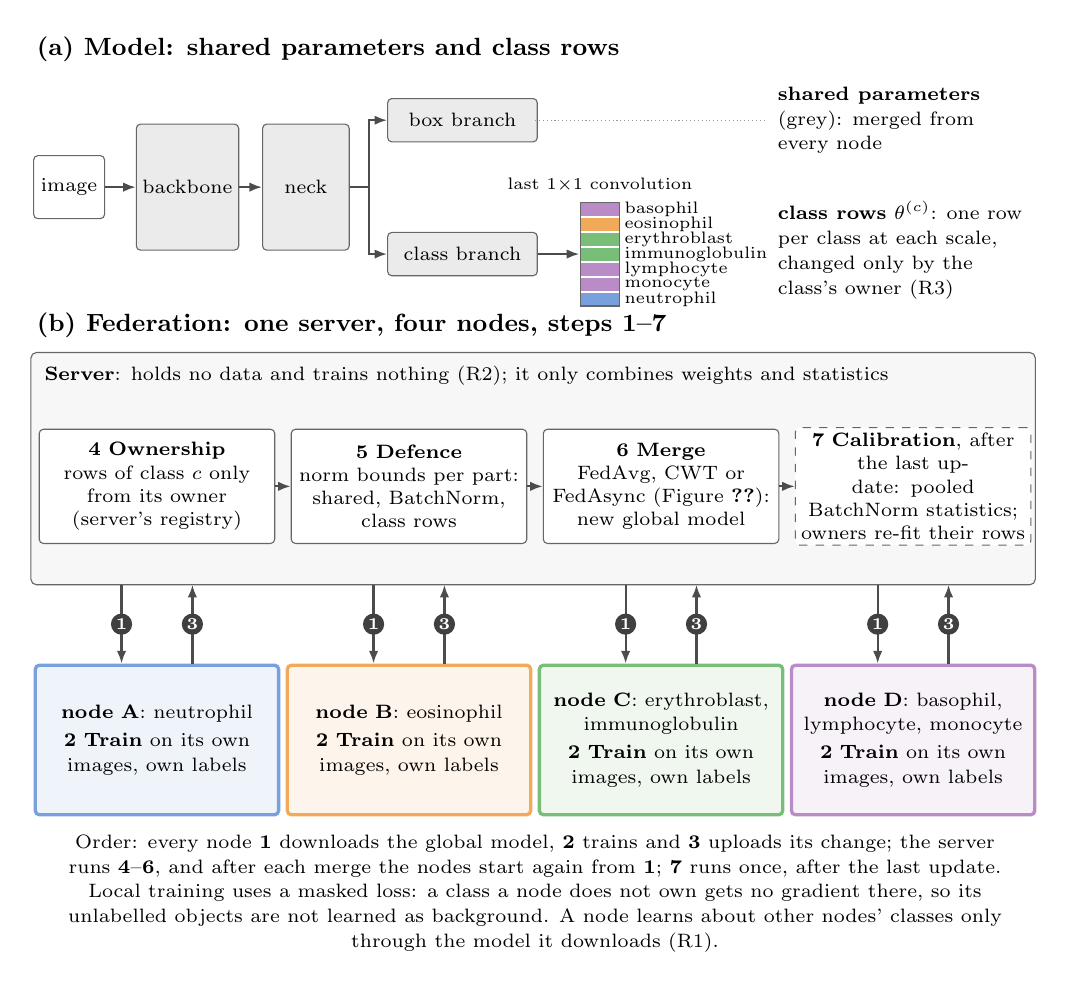
\begin{tikzpicture}[x=0.97cm,y=1cm,font=\fontsize{7.5}{9}\selectfont,
    blk/.style={draw=black!60,rounded corners=1.5pt,align=center,inner sep=2pt},
    shared/.style={blk,fill=black!8},
    stage/.style={blk,fill=white,text width=2.85cm,minimum height=1.45cm,font=\fontsize{7}{8.4}\selectfont},
    arr/.style={-{Latex[length=1.6mm]},black!70,thick},
    num/.style={circle,fill=black!75,text=white,inner sep=0.7pt,font=\fontsize{6.5}{6.5}\selectfont\bfseries}]
  \definecolor{nA}{RGB}{120,160,220}\definecolor{nB}{RGB}{240,170,90}
  \definecolor{nC}{RGB}{120,190,120}\definecolor{nD}{RGB}{185,140,200}
  % ── (a) the model: shared parameters and class rows ──────────────────────────
  \node[anchor=west,font=\fontsize{9}{11}\selectfont\bfseries] at (-0.1,3.05) {(a) Model: shared parameters and class rows};
  \node[blk,minimum width=0.9cm,minimum height=0.8cm] (img) at (0.45,1.3) {image};
  \node[shared,minimum width=1.3cm,minimum height=1.6cm] (bb) at (2.0,1.3) {backbone};
  \node[shared,minimum width=1.1cm,minimum height=1.6cm] (neck) at (3.55,1.3) {neck};
  \node[shared,minimum width=1.9cm,minimum height=0.55cm] (box) at (5.6,2.15) {box branch};
  \node[shared,minimum width=1.9cm,minimum height=0.55cm] (cls) at (5.6,0.45) {class branch};
  \draw[arr] (img) -- (bb); \draw[arr] (bb) -- (neck);
  \draw[arr] (neck.east) -- ++(0.25,0) |- (box.west); \draw[arr] (neck.east) -- ++(0.25,0) |- (cls.west);
  \foreach \col/\lab [count=\i from 0] in {nD/basophil,nB/eosinophil,nC/erythroblast,nC/immunoglobulin,
                                           nD/lymphocyte,nD/monocyte,nA/neutrophil} {
    \fill[\col] (7.15,1.1-\i*0.19) rectangle (7.65,1.1-\i*0.19-0.17);
    \node[anchor=west,font=\fontsize{6}{7}\selectfont,inner sep=1pt] at (7.68,1.1-\i*0.19-0.085) {\lab};
  }
  \draw[black!60] (7.15,1.1) rectangle (7.65,1.1-7*0.19+0.02);
  \draw[arr] (cls.east) -- (7.13,0.45);
  \node[anchor=south,font=\fontsize{6}{7}\selectfont] at (7.4,1.12) {last $1{\times}1$ convolution};
  \node[align=left,anchor=west] at (9.6,2.15) {\textbf{shared parameters}\\(grey): merged from\\every node};
  \node[align=left,anchor=west] at (9.6,0.5) {\textbf{class rows} $\theta^{(c)}$: one row\\per class at each scale,\\changed only by the\\class's owner (R3)};
  \draw[black!40,densely dotted] (6.55,2.15) -- (9.55,2.15);
  % ── (b) the federation, steps numbered in the order they happen ─────────────
  \node[anchor=west,font=\fontsize{9}{11}\selectfont\bfseries] at (-0.1,-0.45) {(b) Federation: one server, four nodes, steps 1--7};
  \draw[black!60,rounded corners=2pt,fill=black!3] (-0.05,-3.75) rectangle (13.1,-0.8);
  \node[anchor=north west,align=left] at (0.0,-0.85) {\textbf{Server}: holds no data and trains nothing (R2); it only combines weights and statistics};
  \node[stage] (s1) at (1.6,-2.5) {\textbf{4 Ownership}\\rows of class $c$ only\\from its owner\\(server's registry)};
  \node[stage] (s2) at (4.9,-2.5) {\textbf{5 Defence}\\norm bounds per part:\\shared, BatchNorm,\\class rows};
  \node[stage] (s3) at (8.2,-2.5) {\textbf{6 Merge}\\FedAvg, CWT or\\FedAsync (Figure~\ref{fig:schemes}):\\new global model};
  \node[stage,dashed] (s4) at (11.5,-2.5) {\textbf{7 Calibration}, after\\the last update: pooled\\BatchNorm statistics;\\owners re-fit their rows};
  \draw[arr] (s1) -- (s2); \draw[arr] (s2) -- (s3); \draw[arr,dashed] (s3) -- (s4);
  % nodes
  \foreach \n/\col/\x/\cls in {A/nA/1.6/{neutrophil},B/nB/4.9/{eosinophil},C/nC/8.2/{erythroblast,\\immunoglobulin},
                                D/nD/11.5/{basophil,\\lymphocyte, monocyte}} {
    \node[blk,draw=\col,very thick,fill=\col!12,text width=2.95cm,minimum height=1.9cm,anchor=north] (n\n) at (\x,-4.75)
      {\textbf{node \n}: \cls\\[1pt]\textbf{2 Train} on its own\\images, own labels};
  }
  \foreach \n in {A,B,C,D} {
    \draw[arr] ([xshift=-0.45cm]n\n.north |- 0,-3.75) -- ([xshift=-0.45cm]n\n.north) node[num,midway] {1};
    \draw[arr] ([xshift=0.45cm]n\n.north) -- ([xshift=0.45cm]n\n.north |- 0,-3.75) node[num,midway] {3};
  }
  \node[anchor=north,align=center] at (6.55,-6.8) {Order: every node \textbf{1} downloads the global model, \textbf{2} trains and \textbf{3} uploads its change; the server\\runs \textbf{4}--\textbf{6}, and after each merge the nodes start again from \textbf{1}; \textbf{7} runs once, after the last update.\\Local training uses a masked loss: a class a node does not own gets no gradient there, so its\\unlabelled objects are not learned as background. A node learns about other nodes' classes only\\through the model it downloads (R1).};
\end{tikzpicture}

\caption{Overview of \sys{}. (a) The detector's parameters. All of them are shared and merged from every node, except the class rows: the row of each class in the last $1\times1$ convolution of the classification branch, at every scale, which only the class's owner changes (the classes of the WBC use case, coloured by their owner). (b) The federation, with its steps numbered in the order they happen. Each node (1) downloads the global model, (2) trains on its own images with the masked loss and (3) uploads its change to the shared parameters and to its own rows. The server, which holds no data, (4) takes each class's rows only from the owner in its registry, (5) bounds each part of the update and (6) merges it into a new global model with FedAvg, CWT or FedAsync (Figure~\ref{fig:schemes}); the nodes then start again from (1). After the last update, (7) the calibration pools BatchNorm statistics and lets each owner re-fit its rows.}\label{fig:architecture}
\end{figure}

\subsubsection{Model and parameter decomposition}
\sys{} uses an anchor-free YOLO detector~\cite{redmon2016yolo,ultralytics}. The study uses YOLO26~\cite{jocher2026yolo26} at scale~L, about 25~M parameters at 640~px, with the classic decoupled detection head. In this head, the last $1\times1$ convolution of the classification branch at each scale maps features to one logit per class. Row $c$ of these convolutions (weights and bias, at every scale) is the only parameter that is specific to class $c$. We call these the \emph{class rows} $\theta^{(c)}$. Every other parameter is \emph{shared}: backbone, neck, box branch and the rest of the classification branch. Shared parameters are initialized from COCO pre-training~\cite{lin2014coco}; class rows start random.

\subsubsection{Local training}
Node $i$ trains with the detection loss in which the classification term of every unowned class is masked:
\begin{equation}
\mathcal{L}^{(i)}_{\text{cls}}=\sum_{c\in\mathcal{C}}[c\in\mathcal{C}_i]\;\mathrm{BCE}(\hat p_c,y_c).
\end{equation}
An unlabelled object of another class therefore produces no gradient that teaches the model it is background. Local training uses SGD (momentum 0.9, weight decay $5\cdot10^{-4}$, batch 4, 2 local epochs per round or update). The learning rate decays linearly from $8\cdot10^{-4}$ to 1\% of it, driven by the progress of the whole federation. A node's momentum stays on its own machine.

\subsubsection{Aggregation schemes}
Figure~\ref{fig:schemes} illustrates the three schemes. We name them after the methods they follow, FedAvg~\cite{mcmahan2017fedavg}, cyclic weight transfer (CWT)~\cite{chang2018distributed} and FedAsync~\cite{xie2019fedasync}, and use these names throughout; in \sys{}, all three take each class's rows only from its owner.
\begin{itemize}
\item \emph{FedAvg, parallel synchronous.} In each round all nodes train from the same global model. The server waits for all of them, averages the shared parameters weighted by data size, and takes each class row from its owner (R3).
\item \emph{CWT, sequential synchronous.} Nodes train one at a time, in an order the server draws at random for every cycle. Each node starts from the model left by the previous one, and the server applies its update in full. This is synchronous: the server schedules the turns and a cycle needs every node. The final model averages the last four global versions (stochastic weight averaging~\cite{izmailov2018swa}), which removes the bias towards the last node.
\item \emph{FedAsync, concurrent asynchronous.} Nodes train continuously and independently, as fast as their hardware allows. An update computed from version $v_{\text{pull}}$ arrives when the global model is at version $v_{\text{now}}$, with staleness $s=v_{\text{now}}-v_{\text{pull}}$. It is applied at once:
\begin{align}
\theta_{\text{shared}} &\leftarrow \theta_{\text{shared}} + w\,\Delta_{\text{shared}}, & w &= \frac{1}{1+\alpha s},\;\alpha=0.5,\\
\theta^{(c)} &\leftarrow \theta^{(c)} + w\,\Delta^{(c)} &&\text{only for } c\in\mathcal{C}_i,
\end{align}
where $\Delta$ is the node's change from the model it pulled~\cite{xie2019fedasync}. BatchNorm running variances are clamped at zero, because stale deltas can push them negative. The final model averages, over nodes, the global version right after each node's last update. Arrival order thus comes from timing alone, never from a server-side choice.
\end{itemize}

\begin{figure}[t]
\centering
% The three aggregation schemes (included by main.tex, Figure fig:schemes).
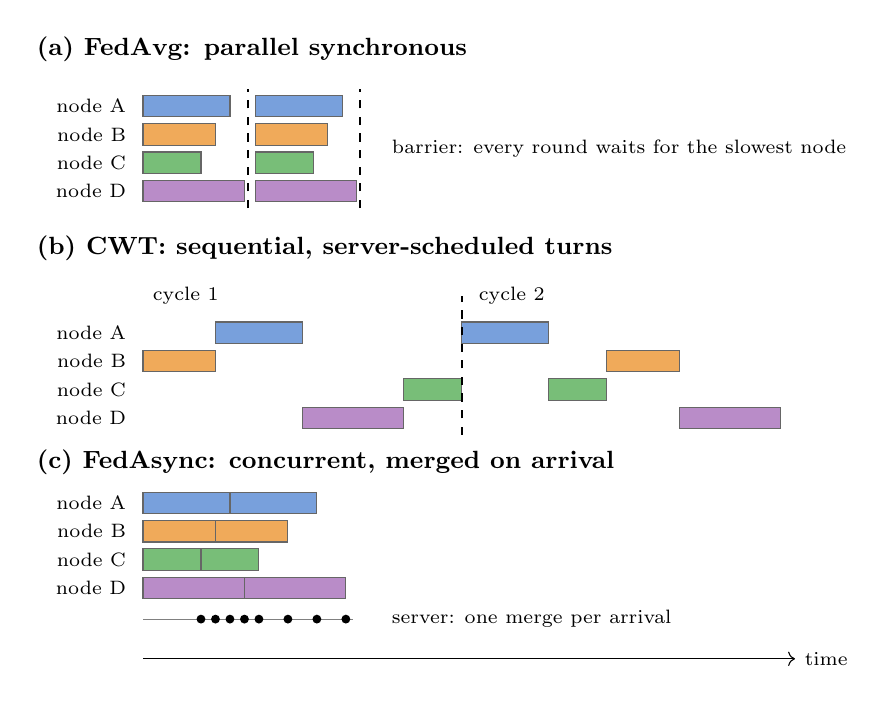
\begin{tikzpicture}[x=0.92cm,y=0.36cm,font=\scriptsize]
  \definecolor{nA}{RGB}{120,160,220}\definecolor{nB}{RGB}{240,170,90}
  \definecolor{nC}{RGB}{120,190,120}\definecolor{nD}{RGB}{185,140,200}
  \newcommand{\job}[4]{\fill[#4] (#1,#3-0.38) rectangle (#2,#3+0.38); \draw[black!60] (#1,#3-0.38) rectangle (#2,#3+0.38);}
  \newcommand{\lanes}[1]{\foreach \n/\y in {A/3,B/2,C/1,D/0} {\node[anchor=east] at (-0.1,#1+\y) {node \n};}}
  % (a) parallel synchronous: lanes 14-17
  \node[anchor=west,font=\small\bfseries] at (-1.6,19.0) {(a) FedAvg: parallel synchronous};
  \lanes{14}
  \foreach \s in {0,1.55} {
    \job{\s}{\s+1.2}{17}{nA}\job{\s}{\s+1.0}{16}{nB}\job{\s}{\s+0.8}{15}{nC}\job{\s}{\s+1.4}{14}{nD}
    \draw[dashed,thick] (\s+1.45,13.4) -- (\s+1.45,17.6);
  }
  \node[anchor=west] at (3.3,15.5) {barrier: every round waits for the slowest node};
  % (b) sequential synchronous: lanes 6-9, cycle labels in their own row above the lanes
  \node[anchor=west,font=\small\bfseries] at (-1.6,12.0) {(b) CWT: sequential, server-scheduled turns};
  \lanes{6}
  \job{0}{1.0}{8}{nB}\job{1.0}{2.2}{9}{nA}\job{2.2}{3.6}{6}{nD}\job{3.6}{4.4}{7}{nC}
  \job{4.4}{5.6}{9}{nA}\job{5.6}{6.4}{7}{nC}\job{6.4}{7.4}{8}{nB}\job{7.4}{8.8}{6}{nD}
  \draw[dashed,thick] (4.4,5.4) -- (4.4,10.3);
  \node[anchor=west] at (0,10.3) {cycle 1}; \node[anchor=west] at (4.5,10.3) {cycle 2};
  % (c) concurrent asynchronous: lanes 0-3
  \node[anchor=west,font=\small\bfseries] at (-1.6,4.45) {(c) FedAsync: concurrent, merged on arrival};
  \lanes{0}
  \job{0}{1.2}{3}{nA}\job{1.2}{2.4}{3}{nA}\job{0}{1.0}{2}{nB}\job{1.0}{2.0}{2}{nB}
  \job{0}{0.8}{1}{nC}\job{0.8}{1.6}{1}{nC}\job{0}{1.4}{0}{nD}\job{1.4}{2.8}{0}{nD}
  \draw[black!50] (0,-1.1) -- (2.9,-1.1); \foreach \t in {0.8,1.0,1.2,1.4,1.6,2.0,2.4,2.8} {\fill (\t,-1.1) circle[radius=1.6pt];}
  \node[anchor=west] at (3.3,-1.1) {server: one merge per arrival};
  \draw[->] (0,-2.5) -- (9,-2.5) node[anchor=west] {time};
\end{tikzpicture}

\caption{The three schemes with four nodes of different speeds, two cycles each. In (a), nodes train in parallel and the server averages after a barrier. In (b), one node trains at a time, starting from the previous node's model, in a new random order every cycle. In (c), nodes train concurrently and each update is merged on arrival. Every scheme trains the same number of node-epochs. CWT needs about three times the wall-clock time (Section~\ref{sec:res-fair}).}\label{fig:schemes}
\end{figure}

\subsubsection{Calibration}\label{sec:calib}
Merging moves the shared features, while each class row was fitted to the features its owner saw. A short \emph{calibration} re-aligns them without breaking R1--R3. Each node computes the BatchNorm statistics of the final model on its own images~\cite{ioffe2015bn}. The server pools them, weighted by batch count, into a mean and variance per channel. Each node then re-fits only its own class rows on the frozen model with the pooled statistics, for one epoch, and the server replaces those rows.

The synchronous form (\emph{closing calibration}) needs a barrier: all statistics, then all rows. We designed a \emph{progressive calibration} for the asynchronous scheme, so that nobody waits. The final model is published at once. Every contribution, as it arrives, makes the server release an updated model. Nodes not yet heard from are represented by the final model's own statistics, weighted by their batch counts, which are known from their training uploads. Once every node has contributed, each re-fits its rows once more on the complete pool. Nodes can download a usable model at any time, and the calibration is complete when every node has been seen. To keep the comparison fair, the centralized reference receives the same calibration.

\subsection{Deployment and defence against malicious nodes}\label{sec:deploy}
The same schemes run in a secured client--server implementation, and the server can screen every upload against a malicious node.

\subsubsection{Networked implementation and security}\label{sec:net}
The schemes evaluated here run unchanged in a client--server implementation. Nodes are client processes, one per site, and the server manages ``rooms'', one per federation. Security measures follow the threats each addresses:
\begin{itemize}
\item \emph{Authentication.} A room password plus a per-node secret token, stored hashed, is required on every request. Administrative actions are allowed only locally or with an admin token.
\item \emph{Safe payloads.} Only plain tensors are exchanged, deserialized without code execution. Every upload is checked against the room's model: same tensor names and shapes, finite values, a size limit, and an idempotent upload identifier.
\item \emph{Ownership.} The server takes class rows only for the classes in its own registry, never for the classes an upload claims (R3).
\item \emph{Transport.} Optional HTTPS, with private certificate authorities supported.
\item \emph{Availability.} Heartbeats mark lost nodes; their turns are skipped in CWT. Requests are retried with back-off, and state is persisted for restarts.
\end{itemize}
Server-side evaluation exists only in a developer mode, because in deployment the server holds no data (R2). CWT is enforced by the server: a node asking out of turn is told to wait. Both schemes and both calibration forms were exercised end to end with a live server and separate client processes on one machine; the code release includes this demonstration for all three use cases \authornote{a multi-machine demonstration would strengthen this paragraph}.

\subsubsection{Ownership-aware robust aggregation}\label{sec:defence}
Byzantine-robust rules compare simultaneous updates and keep the majority view~\cite{blanchard2017krum,yin2018byzantine}. Under disjoint ownership this fails in three ways:
\begin{itemize}
\item a class row has a single contributor, so no majority exists;
\item honest updates of shared layers differ by design, because each node optimizes a different objective;
\item in CWT and FedAsync the server sees one update at a time.
\end{itemize}
Defences that use server data are excluded by R2. We therefore bound what each update can do, part by part, against references the attacker cannot set alone (Algorithm~\ref{alg:ora}):
\begin{itemize}
\item Ownership is enforced from the registry.
\item Each part of an update is scaled down if it exceeds $\kappa=2$ times the median size of that part in the other nodes' recent updates. The parts are the shared weights, the BatchNorm statistics, and each owned class row; class rows have no peers, so their reference pools every node's row sizes.
\item The reference requires updates from at least three other nodes, so with one attacker among four it is set by an honest node.
\item In FedAvg rounds, the shared deltas are combined by a coordinate-wise trimmed mean instead of the data-weighted mean, because reported data sizes are not trusted.
\end{itemize}
Every decision is logged for audit. The bounds limit the size of an update, not its direction; Section~\ref{sec:res-robust} shows the consequence.

\begin{algorithm}[t]
\caption{Ownership-aware screening of one upload from node $i$}\label{alg:ora}
\begin{algorithmic}[1]
\Require upload $\theta_i$, model it was trained from $\theta^{\text{pull}}$, registry $\mathcal{C}_i$, histories $H_p$ of recent part sizes per node
\State $\Delta \gets \theta_i-\theta^{\text{pull}}$; \quad owned classes $\gets \mathcal{C}_i$ \Comment{never the classes the upload claims}
\For{each part $p\in\{\text{shared},\ \text{BatchNorm}\}\cup\{\text{row } c: c\in\mathcal{C}_i\}$}
  \State $b_p \gets \kappa\cdot\operatorname{median}_{j\neq i}\operatorname{median}(H_p^{\,j})$ \textbf{if} $|\{j\neq i\}|\ge 3$ \textbf{else} $\infty$
  \State $\Delta_p \gets \Delta_p\cdot\min\!\left(1,\ b_p/\lVert\Delta_p\rVert\right)$; \quad append $\lVert\Delta_p\rVert$ to $H_p^{\,i}$; \quad log $(i,p,\lVert\Delta_p\rVert,b_p)$
\EndFor
\State \Return $\theta^{\text{pull}}+\Delta$ to the scheme's merge rule
\end{algorithmic}
\end{algorithm}

\subsection{Use cases}\label{sec:usecases}
Table~\ref{tab:datasets} lists the three use cases, and Table~\ref{tab:classes} their classes, owners and instances:
\begin{itemize}
\item \emph{KFM12}: twelve classes of parasite eggs in animal faecal samples, imaged with the Kubic FLOTAC Microscope~\cite{cringoli2021kfm}, the device for which the AI-KFM detectors were developed~\cite{capuozzo2024aikfm,capuozzo2026ijp} \authornote{acquisition details, citation of the released dataset};
\item \emph{WBC}: seven white-blood-cell classes, with bounding boxes~\cite{wbcdetection} on the PBC dataset~\cite{acevedo2020pbc};
\item \emph{DENTEX}: the 32 tooth classes of the enumeration subset~\cite{hamamci2023dentex}. It entered the study after the development phase and is part of every analysis from the confirmatory study on (Section~\ref{sec:protocols}).
\end{itemize}

The three use cases were chosen to cover the conditions a class-owned federation can meet (Table~\ref{tab:datasets}, Figure~\ref{fig:usecases}). Classes share an image never in WBC, sometimes in KFM12 and always in DENTEX. The classes are strongly imbalanced in KFM12, mildly in WBC and nearly uniform in DENTEX. Two use cases are microscopy, with 12 and 7 classes, and one is radiography, with 32.

Each dataset is split once, at image level, into training images (80\%) and an evaluation set (20\%). Classes are assigned greedily to four nodes so that labelled instances are balanced. Every training image goes to each node owning a class present in it, labelled only for that node's classes. Every scheme and the centralized reference train on the same images: for KFM12 and WBC, a class-stratified tenth of the training images, drawn with the seed, so that the three use cases train on a comparable number of images; DENTEX has only 508 training images and trains on all of them. The other training images are not used. The evaluation set is fully labelled, deduplicated and never subsampled, and every model is scored on it.

A WBC image is a crop around a single cell: one object of one class, so no node ever sees an object of another node's class. A KFM12 image holds 2.5 eggs on average, usually of one species (1.1 classes per image), and about a fifth of a node's images also contain eggs of species owned by other nodes. A DENTEX panoramic radiograph shows 29 teeth on average, each of them a class of its own, so every image contains classes of all four nodes: every node holds every image, with only its own eight teeth labelled and the other 24 unlabelled. This is the extreme of disjoint ownership. The masked loss (Section~\ref{sec:system}) keeps those unlabelled teeth from being learned as background, so nothing has to be hidden in the images, and the centralized reference trains on the same partial labels, so \fedcent{} measures the cost of federation alone. The class frequencies differ as well (Table~\ref{tab:classes}). KFM12 is strongly imbalanced: per seed, its commonest class has 669 labelled eggs and its rarest 5. WBC is mildly imbalanced (75--255 cells per class), and DENTEX is nearly uniform (262--506 per tooth, the third molars being the rarest).

\begin{figure}[t]
\centering
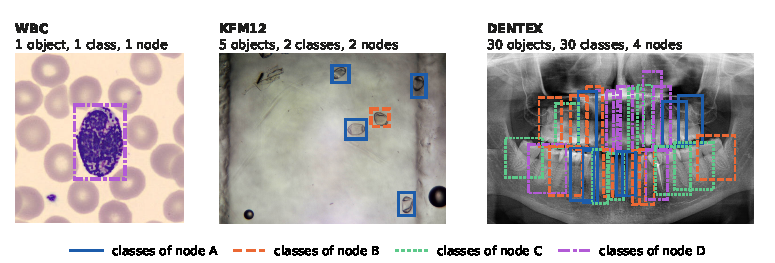
\includegraphics[width=\textwidth]{figures/usecases.pdf}
\caption{One evaluation image of each use case with every labelled object, coloured by the node that owns its class (node colours as in Figures~\ref{fig:architecture} and~\ref{fig:schemes}). WBC: one cell, one class. KFM12: a few eggs, of the species of one or two nodes. DENTEX: every tooth is a class, and every node's classes appear in every radiograph. Images are chosen by a fixed rule (\texttt{tools/make\_usecase\_figure.py}).}\label{fig:usecases}
\end{figure}

\begin{table}[t]
\caption{Use cases. Train: unique images every scheme and the centralized reference train on, per seed (KFM12: 1,385--1,400 over the confirmation seeds). Eval: the fully labelled evaluation set every model is scored on. Objects and classes per image: means over the evaluation set. Unlabelled objects: share of a node's training images that also contain objects of classes owned by other nodes, which that node sees without labels (mean over nodes). Imbalance: labelled instances trained on of the commonest class over those of the rarest. Budget: training epochs, set from where a centralized pilot run's mAP50 plateaus (Section~\ref{sec:protocol}).}\label{tab:datasets}
\footnotesize
\setlength{\tabcolsep}{2.5pt}
\newcommand{\hd}[1]{\begin{tabular}[b]{@{}c@{}}#1\end{tabular}}
\begin{tabular*}{\textwidth}{@{\extracolsep\fill}l>{\raggedright\arraybackslash}p{0.15\textwidth}rrrrrrrr}
\toprule
Use case & Images & Classes & Train & Eval & \hd{Objects\\per image} & \hd{Classes\\per image} & \hd{Unlabelled\\objects} & Imbalance & Budget \\
\midrule
KFM12 & microscopy, parasite eggs & 12 & 1,390 & 3,089 & 2.5 & 1.1 & 22\% & 134$\times$ & 30 \\
WBC & microscopy, blood cells & 7 & 1,068 & 2,668 & 1.0 & 1.0 & 0\% & 3.4$\times$ & 20 \\
DENTEX & panoramic X-ray, teeth & 32 & 508 & 126 & 28.7 & 28.7 & $\approx$100\% & 1.9$\times$ & 20 \\
\botrule
\end{tabular*}
\end{table}

\begin{table}[t]
\caption{Classes, their owner node and their labelled instances: trained on (mean over the ten confirmation seeds; KFM12 and WBC train on a class-stratified tenth of their training images, DENTEX on all of them) and in the evaluation set. KFM12 class names as labelled in the dataset.}\label{tab:classes}
\footnotesize
\setlength{\tabcolsep}{3pt}
\begin{tabular*}{\textwidth}{@{\extracolsep\fill}lcrr@{\hspace{10pt}}lcrr}
\toprule
\multicolumn{4}{c}{\emph{KFM12}} & \multicolumn{4}{c}{\emph{WBC}} \\
\cmidrule(lr){1-4}\cmidrule(lr){5-8}
Class & Owner & Train & Eval & Class & Owner & Train & Eval \\
\midrule
strongili & C & 620 & 1,350 & basophil & D & 88 & 196 \\
fasciola & B & 611 & 1,553 & eosinophil & B & 235 & 579 \\
eimeria intricata & A & 5 & 16 & erythroblast & C & 75 & 176 \\
calicophoron & A & 669 & 2,034 & immunoglobulin & C & 214 & 553 \\
nematodirus & C & 132 & 353 & lymphocyte & D & 93 & 233 \\
dicrocoelium & B & 22 & 58 & monocyte & D & 108 & 279 \\
metastrongili & B & 32 & 55 & neutrophil & A & 255 & 652 \\
strongyloides & C & 106 & 187 &  & & &  \\
moniezia benedeni & A & 34 & 90 &  & & &  \\
ascaris & D & 533 & 1,248 &  & & &  \\
ancylostoma & D & 251 & 627 &  & & &  \\
trichuris trichiuria & B & 120 & 265 &  & & &  \\
\botrule
\end{tabular*}

\medskip
\noindent\emph{DENTEX}: 32 teeth in FDI numbering, eight per node; train and eval: range over a node's eight teeth.\par\smallskip
\begin{tabular*}{\textwidth}{@{\extracolsep\fill}clrr}
\toprule
Owner & Teeth & Train & Eval \\
\midrule
A & 14, 26, 27, 28, 31, 32, 44, 45 & 282--505 & 85--125 \\
B & 13, 15, 17, 33, 34, 38, 42, 46 & 312--506 & 82--124 \\
C & 16, 22, 23, 36, 37, 41, 43, 48 & 319--506 & 83--124 \\
D & 11, 12, 18, 21, 24, 25, 35, 47 & 262--503 & 79--125 \\
\botrule
\end{tabular*}
\end{table}

%=====================================================================================
\section{Experimental design}\label{sec:design}

The experiments separate finding the schemes from testing them. All arms share one training protocol (Section~\ref{sec:protocol}). The schemes were found in an exploratory development phase and then tested once in a confirmatory study registered before its first run (Section~\ref{sec:protocols}). Secondary analyses describe who bears the cost of federation and what it costs to run, and compare the schemes with standard methods and two baselines (Section~\ref{sec:secondary}). A separate study measures robustness to a malicious node (Section~\ref{sec:robust-method}).

Generative AI was used in this work as follows. The authors designed the system architecture, the study and its experiments. Claude Opus 5.5 (Anthropic) was used to draft the manuscript, to develop part of the code, and to automate the experimental runs. The code it developed implements components conceived and designed by the authors, who also validated it. The authors reviewed and verified all content and take full responsibility for it. No AI-generated images are included.

\subsection{Training protocol}\label{sec:protocol}
All arms use the same recipe: 2 local epochs per round or update, and linear learning-rate decay to 1\% over the whole budget. The budget comes from a centralized pilot run of up to 100 epochs, scored every 5 epochs. It is the peak of the three-point moving average of the pilot's mAP50: 30 epochs for KFM12. WBC and DENTEX plateau by the first checkpoint (epoch 5), and keep the 20 epochs of the original protocol. From epoch 5 on, their pilot curves stay within 0.045 and 0.02 mAP50 of their best, with no trend. The budgets correspond to 15, 10 and 10 rounds or updates per node on KFM12, WBC and DENTEX. During development we found that a constant learning rate made the score of a single run swing by $\pm0.02$ mAP50 between checkpoints five epochs apart. That noise was as large as the effects being measured, and decaying the rate halved the seed-to-seed spread of the centralized model.

Concurrency is simulated on one GPU with a seeded discrete-event clock:
\begin{itemize}
\item each node draws a machine speed $1\pm U(0,0.3)$ per seed;
\item an update lasts (images $\times$ epochs) / speed, $\times(1\pm U(0,0.2))$ jitter;
\item updates are applied in the order in which they finish on that clock;
\item each training is executed when its pull happens, so staleness and arrival order are exactly those of the timeline (average staleness 2.4--2.7).
\end{itemize}

\subsection{Development phase and confirmatory study}\label{sec:protocols}
The schemes were chosen in an exploratory phase and then tested once, unchanged, under a registered protocol.

\subsubsection{Exploratory development phase}\label{sec:dev}
The schemes were found by an exploratory search of about 30 variants on seeds 0--3. The variants changed aggregation rules, update strength, losses, calibration and execution order (listed in the released search report). The development phase itself had a pre-registered protocol with a 90\% margin, and its threshold was later lowered to 85\% after results were seen. Because the margin was set after seeing data and the schemes were chosen on the evaluation seeds, development-phase bounds are optimistic (winner's curse). We report them as exploratory only.

\subsubsection{Confirmatory study}\label{sec:confirm}
The two final schemes were then confirmed under a protocol registered before its first run:
\begin{itemize}
\item \emph{Schemes:} CWT with closing calibration, and FedAsync with progressive calibration and refresh.
\item \emph{Seeds:} ten seeds never used before (100--109). Each seed also draws the node order of CWT, the machine speeds of FedAsync and the training subsets.
\item \emph{No early stopping and no added seeds.}
\item \emph{Margins:} tested in a fixed sequence~\cite{wiens2003fixed}: 85\% then 90\% for the synchronous scheme, 80\% then 85\% for the asynchronous one. The claim is the last margin passed.
\item \emph{Frozen artefacts:} the analysis script, configurations and code were frozen in a separate copy and recorded by SHA-256 before the first run, and the study runs from that copy.
\item \emph{Third use case:} DENTEX was added after the development phase, with criteria fixed in advance (public, at least 8 classes, a new modality, licensed for research). It was named in a dated amendment before its first run. A second amendment, also before any DENTEX run, made the headline claim cover every registered use case, DENTEX included. A third amendment fixed DENTEX's budget from its centralized pilot. It was made before any federated DENTEX run, and it corrected the registered description of the budget rule, which did not match how the study budgets had been set (Section~\ref{sec:protocol}).
\end{itemize}
Planning simulations from the development data gave a power above 0.95 for the synchronous scheme at 85\% and the asynchronous scheme at 80\%, but only about 0.67 for the asynchronous scheme at 85\%.

\subsection{Secondary analyses and baselines}\label{sec:secondary}
\begin{itemize}
\item \emph{Fairness:} per-class retention (federated AP50 / centralized AP50 of the class, means over seeds), the worst class, the number of classes below 85\%, retention per node, and its Spearman correlation with the number of training boxes of the class (permutation $p$-values).
\item \emph{Cost:} GPU time and energy, measured from the GPU's power draw; communication volume; and deployment wall-clock from the timing model.
\item \emph{Standard methods:} FedProx~\cite{li2020fedprox}, FedBuff~\cite{nguyen2022fedbuff} and CA2FL~\cite{wang2024ca2fl}, under the same protocol and post-processing, on the development seeds of KFM12 and WBC.
\item \emph{Local-only baseline (exploratory, after the confirmatory study):} each node trains a detector alone on its own data and classes, with the same recipe and the same number of epochs it trains in the federation, and each class is scored on its owner's model, as if every class were reported by its owner. It measures what federation adds over not federating. Seeds 100--102 on all three use cases.
\item \emph{Centralized reference with weight averaging (exploratory):} on WBC, the centralized model trained with the averaging of CWT (the mean of four snapshots over the last two epochs, one every half epoch, as one sequential turn trains on a quarter of the data for two epochs), then calibrated. Seeds 100--109. It tests whether averaging explains why the federated schemes score above centralized on WBC (Section~\ref{sec:res-cost-fed}).
\end{itemize}

\subsection{Robustness study}\label{sec:robust-method}
Table~\ref{tab:attacks} lists the attacks, and Figure~\ref{fig:attacks} shows them on images of the three use cases. The study runs on WBC, the use case with the shortest runs, so that its 120 runs fit the compute budget. With seeds 0--2 and the attacker rotating with the seed, each attack is run on each scheme with and without the defence, and the defence is also run on clean federations to measure its cost. Models are scored as the server evaluates them after the last update, that is, the last global version, without calibration. We report mAP50 and \fedcent{}, mAP50 on the attacker's classes and on everyone else's, and the share of uploads the defence scaled, for the attacker and for honest nodes. For the backdoor we also report the attack success rate: the share of triggered evaluation images on which the target class is detected on the trigger, at confidence $\ge0.25$ and IoU $\ge0.5$.

Standard evaluation keeps at most 300 detections per image after non-maximum suppression, shared by all classes. A class whose scores are high everywhere can fill that budget and leave none to the others. To measure this effect, the defended sign-flip runs and the FedAsync BatchNorm-poisoning seed that collapsed were repeated with their final model kept, and these models and the defended clean runs are also scored with a \emph{per-class budget}, in which every class keeps its own 300 detections. When no class fills the shared budget, the two evaluations give identical results.

After these results, we tested four candidate defences against the attacks the defence did not stop. All are exploratory, and all keep the rules of Section~\ref{sec:problem}: the server holds no data, and only a class's owner changes its rows.
\begin{itemize}
\item \emph{Median pooling of BatchNorm statistics in the calibration.} The calibration discards the BatchNorm statistics accumulated in training and pools those the nodes compute on their own images (Section~\ref{sec:calib}). The registered rule weights each node's statistics by its batch count. The candidate takes their coordinate-wise median~\cite{yin2018byzantine}, which one node among four cannot move outside the range of the honest ones. Unlike class rows, BatchNorm statistics come from every node, so they can be compared; corrupted statistics are known to break federated training~\cite{guerraoui2024bn}. We apply the BatchNorm step alone to the final models of the BatchNorm-poisoning runs, repeated with their final model kept, and of the defended clean runs. Every node is honest in the calibration, or the attacker also poisons the statistics it sends, with the corruption of Table~\ref{tab:attacks}.
\item \emph{Screening inputs at the nodes.} Detector Cleanse~\cite{chan2022baddet} checks a detection at inference by blending the detected region with crops of other objects. A trigger keeps its class whatever is blended in, so the entropy of the class scores stays abnormally low. A node blends each detection with 32 of 64 crops of its own labelled objects (weight 0.5) and normalizes the sigmoid class scores before computing the entropy. It checks the detections of classes it does not own, and flags those whose average entropy falls below the 5th percentile of the entropies of the detections on its own validation images. This threshold was fixed after two pilot rules, on 10--20 images of seeds 0 and 1, flagged too many clean images. The screening node is the honest node after the attacker. We measure the attack success rate on 100 triggered evaluation images with and without screening, the share of the same images without the trigger that are flagged (false alarms), and the AUROC of the entropy between the backdoor's detections and the checked detections on clean images.
\item \emph{Bounding consecutive merges jointly in FedAsync.} The updates a node merges in a row, with no other node's update in between, are bounded together for the shared weights and the BatchNorm statistics: their cumulative change must stay within the bound of one update. Per-update bounds cannot stop a direction that persists when no honest update follows, as in the concurrent seed whose attacker sent its last three uploads in a row. We run it on the FedAsync BatchNorm-poisoning runs and on clean FedAsync runs, with the defence, seeds 0--2.
\item \emph{Peer validation with per-class rollback.} After every new global version, each node runs the model on 32 of its own training images, without labels, and reports one number per class: the share of the head's locations where the class scores at least 0.25. A node votes against a class that covers at least 2\% of the locations on its images and at least ten times the median of the other classes there; its owner does not vote on it. A class flagged by a majority of the nodes that do not own it at two checks in a row is rolled back to its rows at the last check it passed, and its owner's later row updates are discarded~\cite{andreina2021baffle}. Its rows thus only ever hold values its owner produced (R3): the other nodes can veto them, never write them. The node named as attacker also lies in its reports, so the vote itself is tested. The thresholds were set on the kept final models of the robustness study before any of these runs: clean and backdoored classes cover at most 0.1\% of the locations, the sign-flipped class 16--90\%. We run it on the sign-flip runs with the defence and on clean runs, in the three schemes, seeds 0--2.
\end{itemize}

\begin{table}[t]
\caption{Attacks. One node of four is the attacker. Data attacks change the attacker's training data; upload attacks change what it sends.}\label{tab:attacks}
\footnotesize
\begin{tabular*}{\textwidth}{@{\extracolsep\fill}>{\raggedright\arraybackslash}p{0.18\textwidth}>{\raggedright\arraybackslash}p{0.50\textwidth}>{\raggedright\arraybackslash}p{0.22\textwidth}}
\toprule
Attack & What the attacker does & Detection-specific \\
\midrule
noise & sends Gaussian noise, $3\times$ its honest update's size, tensor by tensor (faulty node) & no \\
sign flip & sends the opposite of its honest update, same size & no \\
scaling & boosts its update $\times10$ (model replacement~\cite{bagdasaryan2020backdoor}) & no \\
weight inflation & reports $100\times$ its image count (FedAvg weights) & no \\
BatchNorm poisoning & shifts running means by $3\sigma$, scales variances $\times9$ & yes: statistics shared by every class \\
row hijacking & claims every class, makes others' classes fire everywhere & yes: per-class rows \\
box corruption & drops half its boxes, moves and resizes the rest & yes \\
phantom-object backdoor & checkerboard trigger in 30\% of its images, labelled as its class~\cite{chan2022baddet} & yes \\
\botrule
\end{tabular*}
\end{table}

\begin{figure}[!tbp]
\centering
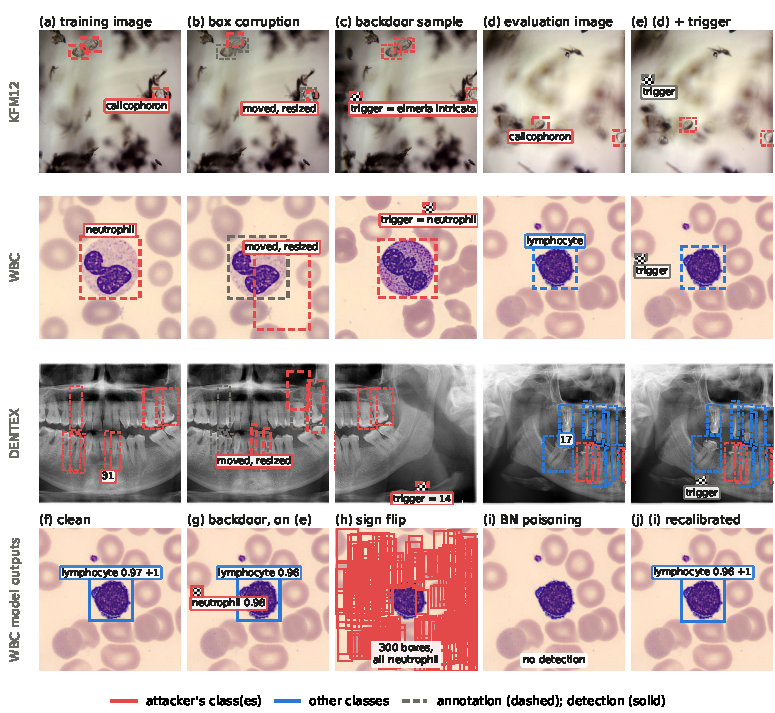
\includegraphics[width=\textwidth]{figures/attacks.pdf}
\caption{Attacks of the robustness study. Rows 1--3: the data attacks on a KFM12, a WBC and a DENTEX image, with node A, the attacker of seed 0, whose classes are in red. (a) One of its training images with its boxes; (b) the same image with corrupted labels: half the boxes dropped (grey only), the others moved and resized; (c) a backdoor sample, with the trigger labelled as the attacker's first class; (d) an evaluation image without that class and (e) the same image with the trigger. The WBC panels come from the study's attack data; KFM12 and DENTEX, on which the robustness study was not run, apply the same rules. Panels are square crops as wide as the image's short side (for DENTEX, the central part of the radiograph). Row 4: what federations trained under attack detect. The robustness study trained them on WBC only, so these outputs exist only for WBC: detections (confidence $\ge0.25$) of final models trained with the defence: (f) clean federation on (d); (g) backdoored federation on (e); (h) sign flip on (d), where the attacker's class fills the budget of 300 detections; (i) BatchNorm poisoning in the FedAsync seed that collapsed (attacker node C), final model before calibration, on (d); (j) the model of (i) after the BatchNorm step of the calibration with median pooling, the attacker also poisoning the statistics it sends. Each object shows its most confident detection; $+k$ counts the other classes detected on it at lower confidence, as models trained on partial labels do. Images are chosen by a fixed rule (first match in file order).}\label{fig:attacks}
\end{figure}

%=====================================================================================
\section{Results}\label{sec:results}

We first report the cost of federation: the exploratory development phase, then the registered confirmatory test on the three use cases (Section~\ref{sec:res-cost-fed}). We then show who bears that cost and what each scheme costs to run (Section~\ref{sec:res-fair}), compare the schemes with standard methods and a local-only baseline (Section~\ref{sec:res-baselines}), and report the robustness study (Section~\ref{sec:res-robust}).

\subsection{The cost of federation}\label{sec:res-cost-fed}
We report the development phase, on KFM12 and WBC, and the confirmatory test, on the three use cases.

\subsubsection{Development phase}\label{sec:res-explore}
Table~\ref{tab:explore} summarizes the development phase under the final protocol on KFM12 and WBC:
\begin{itemize}
\item On both, every scheme is within about 10\% of centralized or above it.
\item CWT is the closest on KFM12 (102\%).
\item Calibration helps FedAsync most: from 89\% to 95\% on KFM12.
\end{itemize}
Two lessons from this phase bear on trustworthy evaluation in general:
\begin{itemize}
\item \emph{Results that depended on execution order were taken as method effects.} Earlier ``asynchronous'' results had been obtained with one node training at a time. With real concurrency the conclusions changed.
\item \emph{A winner did not survive confirmation.} An asynchronous scheme that passed on development seeds failed on fresh seeds (lower bound 89.8\% against a 90\% margin), and we withdrew it.
\end{itemize}

\begin{table}[t]
\caption{Development phase (exploratory, protocol of Section~\ref{sec:protocol}): \fedcent{} mean over seeds, with the lower end of its 95\% CI in parentheses. Calibrated rows are compared with the centralized model given the same calibration. These bounds were obtained on the seeds used to choose the schemes and are optimistic. DENTEX entered the study after this phase, so it has no development runs.}\label{tab:explore}
\footnotesize
\begin{tabular*}{\textwidth}{@{\extracolsep\fill}llccc}
\toprule
Scheme & Post-processing & $n$ & KFM12 & WBC \\
\midrule
FedAvg & none & 3 & 94.6 (82.9) & 111.9 (84.5) \\
 & closing calibration & 3 & 94.0 (79.6) & 114.8 (94.2) \\
CWT & none & 3 & 101.6 (87.9) & 106.4 (82.2) \\
 & closing calibration & 3 & 102.1 (85.7) & 111.0 (98.8) \\
FedAsync & none & 4 & 89.1 (82.4) & 106.4 (81.3) \\
 & progressive calibration & 4 & 94.6 (89.2) & 111.9 (85.6) \\
 & progressive + refresh & 4 & 95.0 (89.8) & 114.0 (86.9) \\
\midrule
\multicolumn{3}{l}{Centralized mAP50 (seeds 0--3)} & 0.734 & 0.548 \\
\botrule
\end{tabular*}
\end{table}

\subsubsection{Confirmatory study}\label{sec:res-confirm}
Table~\ref{tab:confirm} gives the confirmatory results on KFM12, WBC and DENTEX. The registered test, run once on all ten seeds, requires the lower bound to exceed the margin on every use case it covers. It is applied to the use cases registered first, to DENTEX on its own, as the amendment that added it registered, and, as the headline claim (amendment 2), to every registered use case:
\begin{itemize}
\item \emph{CWT.} It passes both margins of its fixed sequence, 85\% and 90\%, in every test, so its claim is 90\% on every registered use case. Its lower bounds are 96.7\% on KFM12, 98.7\% on WBC and 96.2\% on DENTEX.
\item \emph{FedAsync.} Its lower bounds are 92.1\% on KFM12, 122.0\% on WBC and 99.4\% on DENTEX. On DENTEX, tested on its own as registered, it passes both of its margins, 80\% and 85\%. Read post hoc over the three use cases reported here, every lower bound exceeds 90\%; this reading is not the registered test, whose sequence for this scheme stops at 85\%. \authornote{registered verdict of FedAsync over the use cases registered first and over every registered use case: to be written by the authors}
\end{itemize}

\begin{table}[t]
\caption{Confirmatory study (seeds never used in development, frozen code and configurations). \fedcent{}: federated / centralized mAP50 $\times100$, paired by seed, both after the same post-processing; mean, standard deviation and two-sided 95\% $t$-interval. Loss: centralized minus federated mAP50, mean with its upper 95\% bound. mAP50-95: the same ratio for mAP50-95, with its lower bound.}\label{tab:confirm}
\footnotesize
\setlength{\tabcolsep}{3pt}
\begin{tabular*}{\textwidth}{@{\extracolsep\fill}llccccc}
\toprule
Scheme & Use case & $n$ & \fedcent{} (sd) & 95\% CI & Loss (upper) & mAP50-95 (low) \\
\midrule
CWT & KFM12 & 10 & 98.6 (2.7) & 96.7--100.6 & +0.010 (+0.025) & 98.6 (96.0) \\
closing calib. & WBC & 10 & 105.4 (9.4) & 98.7--112.1 & $-$0.025 (+0.007) & 105.3 (98.7) \\
 & DENTEX & 10 & 98.8 (3.7) & 96.2--101.4 & +0.012 (+0.037) & 98.6 (95.6) \\
\midrule
FedAsync & KFM12 & 10 & 93.6 (2.0) & 92.1--95.1 & +0.047 (+0.058) & 93.2 (91.4) \\
progressive & WBC & 10 & 130.8 (12.3) & 122.0--139.6 & $-$0.152 ($-$0.114) & 129.8 (121.1) \\
calib. + refresh & DENTEX & 10 & 99.7 (0.5) & 99.4--100.1 & +0.003 (+0.006) & 101.4 (100.6) \\
\midrule
\multicolumn{3}{l}{Centralized mAP50 (calibrated)} & \multicolumn{4}{l}{KFM12 0.734, WBC 0.502, DENTEX 0.959} \\
\botrule
\end{tabular*}
\end{table}

Three features of the results on KFM12 and WBC deserve comment:
\begin{itemize}
\item \emph{Spread.} The seed-to-seed spread is small on KFM12 (sd 2.0--2.7 points), so the lower bounds are close to the means. This is the effect of the protocol's learning-rate decay (Section~\ref{sec:protocol}).
\item \emph{The cost of concurrency on KFM12.} FedAsync costs 0.047 mAP50 (upper bound 0.058), about five times the cost of CWT. Section~\ref{sec:res-fair} shows that this cost falls on rare classes.
\item \emph{WBC above centralized.} Both federated schemes score above centralized on WBC, as they did in development, and FedAsync by about a third.
\end{itemize}
On the last point: WBC saturates earliest. Its centralized pilot does not improve after the first checkpoint (epoch 5), so most of the budget is spent on a plateau. Federated training averages model versions, over the last turns or over nodes, and averaging weights along such a plateau is known to improve generalization~\cite{izmailov2018swa}. We tested this explanation by giving the centralized model the averaging of CWT (Section~\ref{sec:secondary}, seeds 100--109). Averaging raised its calibrated mAP50 from 0.502 to 0.516, to 102.9\% of the plain centralized model (95\% CI 99.2--106.6). Against this averaged reference:
\begin{itemize}
\item \emph{CWT:} 102.5\% (95\% CI 96.2--108.9). Its excess over centralized is within what averaging explains. Before calibration it is below centralized (98.3\%).
\item \emph{FedAsync:} 127.1\% (95\% CI 120.0--134.3). Its excess is already present before calibration (126.0\%), and averaging over time does not explain it. FedAsync also averages across nodes, over each node's latest version, which a single centralized model cannot reproduce; we did not test whether this is the cause.
\end{itemize}
Because the test is one-sided, values above 100\% do not enter the claim, and we do not interpret them as a benefit of federation.

DENTEX tests the system where class ownership is most entangled. Every radiograph is held by all four nodes, each with only its own eight teeth labelled. A node therefore sees the other 24 teeth in every image as unlabelled. The centralized pilot learns the task quickly: mAP50 0.945 after 5 epochs and 0.958 at best (epoch 15). Most of the room for a federation loss is therefore in how the shared features are merged, not in learning each class.

Both schemes stay close to centralized on DENTEX (Table~\ref{tab:confirm}): CWT at 98.8\% (lower bound 96.2\%), FedAsync at 99.7\% (99.4\%). The worst class is at 98\% under CWT and 97\% under FedAsync, and every node keeps 99--100\% (Table~\ref{tab:fair}). Two points qualify this result:
\begin{itemize}
\item \emph{One weak seed.} The CWT interval is wider because of seed 106, on which the CWT model reached 88.4\%, with every class lower rather than a few. The run completed normally, and as registered it counts like any other seed. The other nine seeds are within 1\% of centralized.
\item \emph{Near the ceiling.} With centralized mAP50 at 0.959, little room is left for a loss. DENTEX tests the extreme of entangled ownership on an easy task, not on a hard one.
\end{itemize}

\subsection{Fairness and cost}\label{sec:res-fair}
Mean ratios do not say who bears the cost of federation, nor what each scheme costs to run; we report both.

\subsubsection{Fairness across classes and nodes}
Mean ratios can hide large losses on single classes (Table~\ref{tab:fair}). The CWT and FedAsync rows use the confirmation seeds. FedAvg was not confirmed, so its rows use the development seeds. The development seeds gave the same picture for the other two schemes.
\begin{itemize}
\item \emph{CWT.} It keeps almost every class close to centralized. Its worst class on WBC is at 94\%. On KFM12 only one class in twelve falls below 85\%: eimeria, the rarest, with 50 training boxes, at 75\%. Its paired difference has a confidence interval that includes zero ($-0.107$, 95\% CI $-0.242$ to $+0.028$). Retention on KFM12 still grows with class size ($\rho=+0.63$). On DENTEX its worst class is at 98\%.
\item \emph{FedAsync.} It concentrates its KFM12 loss on the three rarest classes, while its median class is at 98\%: eimeria at 52\%, metastrongili (307 boxes) at 59\% and dicrocoelium (201 boxes) at 69\%. All three paired differences exclude zero. The two nodes that own these classes average 84\% and 81\%; the other two average 95\% and 101\%. On WBC FedAsync scores above centralized on every class (111--168\%), an excess that weight averaging does not explain (Section~\ref{sec:res-confirm}). On DENTEX it keeps every class at 97\% or more and every node at 99--100\%.
\item \emph{FedAvg.} On development seeds it concentrates its losses on rare classes in the same way: worst class 59\% on KFM12, $\rho=+0.73$.
\end{itemize}
A federation that meets a mean-level guarantee can thus still fail the owners of rare classes. DENTEX has no rare class (262--506 training boxes per tooth), and neither scheme loses a class there. Reporting the worst class and the per-node retention next to the mean should be part of the acceptance criteria.

\begin{table}[t]
\caption{Per-class retention (federated AP50 / centralized AP50 of the class, \%, means over seeds, both calibrated). CWT and FedAsync: confirmation seeds ($n=10$). FedAvg: development seeds. $\rho$: Spearman correlation of retention with the class's training boxes.}\label{tab:fair}
\footnotesize
\begin{tabular*}{\textwidth}{@{\extracolsep\fill}llrrrcl}
\toprule
Scheme & Use case & Worst & Median & Below 85\% & Nodes & $\rho$ (boxes) \\
\midrule
CWT & KFM12 & 75 & 100 & 1/12 & 92--101 & $+0.63^{*}$ \\
 & WBC & 94 & 104 & 0/7 & 94--114 & $+0.32$ \\
 & DENTEX & 98 & 99 & 0/32 & 99 & $-0.61^{*}$ \\
FedAsync & KFM12 & 52 & 98 & 3/12 & 81--101 & $+0.59$ \\
 & WBC & 111 & 131 & 0/7 & 126--137 & $-0.11$ \\
 & DENTEX & 97 & 100 & 0/32 & 99--100 & $+0.34$ \\
FedAvg & KFM12 & 59 & 98 & 3/12 & 87--94 & $+0.73^{*}$ \\
(development seeds) & WBC & 89 & 112 & 0/7 & 103--142 & $+0.07$ \\
\botrule
\end{tabular*}
\footnotesize{$^{*}\,p<0.05$ (permutation test, 20,000 permutations; FedAsync on KFM12 and DENTEX: $p=0.05$). Nodes: range of the mean retention of each node's classes. On DENTEX retention spans only 98--100\% (CWT) and 97--102\% (FedAsync), so its correlations describe differences of a few points.}
\end{table}

\subsubsection{Compute, communication and waiting time}
All federated schemes train the same number of node-epochs, so their compute is the same. Every run was trained on one laptop GPU (NVIDIA RTX 3080 Laptop, 8~GB):
\begin{itemize}
\item \emph{Time.} A federated run took a median of 26--62 GPU minutes depending on the use case, plus 4--11 minutes of calibration. This is 1.1--1.4 times the centralized run on the same data, the difference being per-turn overhead.
\item \emph{Energy.} Integrated from the GPU's power draw sampled every 10~s during the confirmation (median 71~W while training), a run used 0.03--0.08~kWh. One seed of all three arms on KFM12, WBC and DENTEX used about 0.52~kWh.
\item \emph{DENTEX.} Every node holds every image, so each image is trained four times per epoch, once by each owner with its own labels. The centralized reference does the same (Section~\ref{sec:problem}), so the two train the same number of image-epochs, as on the other use cases.
\item \emph{Communication.} It is the same for all schemes: one download and one upload of the 99.4~MB model per node and turn, which totals 2.0--3.0~GB per node. The calibration adds 0.28~MB of statistics and rows per node.
\end{itemize}
The schemes differ in waiting time. With the machine speeds of our timing model, CWT needs 2.4--3.3 times the wall-clock time of FedAsync, and FedAvg about the same as FedAsync (1.00--1.03). CWT also exposes each node's individual update to the server. It therefore cannot use secure aggregation~\cite{bonawitz2017secagg}, which hides individual updates from the server and is available to FedAvg.

\subsection{Comparison with standard methods and a local-only baseline}\label{sec:res-baselines}
Table~\ref{tab:baselines} compares the schemes with FedProx~\cite{li2020fedprox}, FedBuff~\cite{nguyen2022fedbuff} and CA2FL~\cite{wang2024ca2fl} on the development seeds. The standard methods run inside the same system, with the same masked loss, class-row ownership, training budget and post-processing; only the rule that combines updates changes. FedProx adds a proximal term ($\mu=0.01$) to FedAvg. FedBuff and CA2FL replace the merge of FedAsync with buffered aggregation, and CA2FL also calibrates each step with a cache of every node's latest update.

\begin{table}[t]
\caption{Comparison with standard methods (development seeds 0--2 for every method on KFM12 and WBC, and seeds 100--102 on DENTEX, which entered after the development phase; so the FedAsync row differs slightly from the four-seed row of Table~\ref{tab:explore}). \fedcent{}: mean, with the lower end of its 95\% CI in parentheses; worst class: retention of the class with the lowest federated / centralized AP50. Post-processing: closing calibration after parallel and sequential training, progressive calibration with refresh after concurrent training, applied to the centralized reference as well. Exploratory: three seeds, no registered test. \pending{DENTEX column, seeds 100--102: queued}}\label{tab:baselines}
\footnotesize
\begin{tabular*}{\textwidth}{@{\extracolsep\fill}llcccc}
\toprule
 & & \multicolumn{2}{c}{KFM12} & \multicolumn{2}{c}{WBC} \\
Method & Execution & \fedcent{} & Worst class & \fedcent{} & Worst class \\
\midrule
\sys{} FedAvg & parallel & 94.0 (79.6) & 59 & 114.8 (94.2) & 89 \\
FedProx & parallel & 93.8 (82.9) & 45 & 123.6 (77.7) & 107 \\
FedBuff & concurrent & 96.3 (81.1) & 47 & 122.6 (90.6) & 107 \\
CA2FL & concurrent & 87.1 (81.7) & 41 & 104.2 (89.0) & 89 \\
\sys{} FedAsync & concurrent & 96.2 (89.3) & 68 & 117.5 (70.4) & 108 \\
\sys{} CWT & sequential & 102.1 (85.7) & 97 & 111.0 (98.8) & 92 \\
\botrule
\end{tabular*}
\end{table}

\begin{itemize}
\item \emph{KFM12.} CWT is the only method above centralized, and the only one that keeps every class above 85\% (worst class 97\%). Every method that merges updates trained in parallel or concurrently loses the rarest class, eimeria, keeping 41--68\% of its centralized AP50. Among the standard methods, FedBuff has the highest mean (96.3\%) and CA2FL the lowest (87.1\%).
\item \emph{WBC.} Every method scores above centralized on average (104--124\%), and with three seeds the confidence bounds overlap widely.
\end{itemize}
Buffering and update caches therefore do not remove the rare-class loss of averaging-based schemes; only server-scheduled turns did. With three seeds and no registered test, this comparison ranks methods only roughly; the confirmatory claims rest on Table~\ref{tab:confirm} alone.

Table~\ref{tab:local} compares training alone with the two federated schemes on the same seeds.

\begin{table}[t]
\caption{Local-only baseline: each node trains alone on its own data and classes, and each class is scored on its owner's model. Seeds 100--102 for every row, so the federated rows differ from the ten-seed values of Tables~\ref{tab:confirm} and~\ref{tab:fair}. Ratios to the calibrated centralized reference of the same seed (\%). \fedcent{}: mean, with the lower end of its 95\% CI in parentheses. Worst class, classes below 85\% and node range as in Table~\ref{tab:fair}. Exploratory: three seeds, no registered test.}\label{tab:local}
\footnotesize
\begin{tabular*}{\textwidth}{@{\extracolsep\fill}llcccc}
\toprule
Use case & Training & \fedcent{} & Worst class & Below 85\% & Nodes \\
\midrule
KFM12 & local only & 89.5 (79.9) & 34 & 4/12 & 75--94 \\
 & CWT & 98.8 (97.6) & 73 & 1/12 & 91--104 \\
 & FedAsync & 93.1 (86.7) & 49 & 3/12 & 77--106 \\
\midrule
WBC & local only & 95.9 (76.0) & 81 & 1/7 & 81--107 \\
 & CWT & 103.1 (89.3) & 81 & 1/7 & 99--127 \\
 & FedAsync & 136.4 (86.0) & 108 & 0/7 & 140--153 \\
\midrule
DENTEX & local only & 99.9 (98.5) & 96 & 0/32 & 99--101 \\
 & CWT & 100.4 (99.1) & 98 & 0/32 & 100--101 \\
 & FedAsync & 99.9 (99.4) & 95 & 0/32 & 99--100 \\
\botrule
\end{tabular*}
\end{table}

\begin{itemize}
\item \emph{KFM12.} Training alone keeps 89.5\% of centralized, against 98.8\% for CWT. The difference falls on the rare classes. Eimeria keeps 34\% of its centralized AP50 when its owner trains alone, 73\% under CWT and 49\% under FedAsync. Under CWT every node keeps more than it does alone (91--104\% against 75--94\%). Under FedAsync one node does not: the owner of dicrocoelium and metastrongili keeps 89\% alone and 77\% in the federation.
\item \emph{WBC.} Training alone keeps 95.9\%, and both schemes score higher. The node that owns neutrophils gains most from federating: 81\% alone, 106\% under CWT. With three seeds the bounds are wide.
\item \emph{DENTEX.} Training alone matches centralized (99.9\%), as both schemes do. Every node holds every radiograph, so each owner already trains on all the images of its teeth. Federation adds no accuracy here, only one detector in place of four.
\end{itemize}
The local-only reference favours not federating. A node that trains alone detects only its own classes, and the scoring above assumes that the four models are exchanged after training and run side by side, at four times the inference cost. Federation adds the most accuracy where classes are rare and spread over nodes, and none where every node sees every image. FedAsync can leave a node worse off than training alone. Each node can check this on its own validation images, by comparing the federated model with one it trained alone on its own classes, without data from the other nodes.

\subsection{Robustness to a malicious node}\label{sec:res-robust}
Table~\ref{tab:robust} summarizes the robustness study.

\begin{table}[t]
\caption{Robustness on WBC: \fedcent{} (\%, mean over seeds 0--2, attacker rotating with the seed), without / with the defence, last global version without calibration. --: not run. Row hijacking is shown with ownership not enforced / enforced, without the other parts of the defence.}\label{tab:robust}
\footnotesize
\begin{tabular*}{\textwidth}{@{\extracolsep\fill}lccc}
\toprule
Attack & CWT & FedAsync & FedAvg \\
\midrule
none (cost of the defence) & 106 / 100 & 109 / 110 & 112 / 103 \\
noise & 80 / 82 & 97 / 98 & -- \\
box corruption & 83 / 82 & 98 / 98 & -- \\
BatchNorm poisoning & 53 / 100 & 75 / 70$^{a}$ & -- \\
scaling $\times10$ & 22 / 84 & 34 / 81 & 34 / 121 \\
weight inflation $\times100$ & -- & -- & 61 / 116 \\
row hijacking & 90 / 101 & 90 / 112 & -- \\
phantom-object backdoor$^{b}$ & 96 / 109 & 114 / 106 & 112 / 110 \\
sign flip & 0 / 0 & 0 / 5 & 0 / 0 \\
sign flip, per-class budget$^{c}$ & -- / 82 & -- / 91 & -- / 96 \\
\botrule
\end{tabular*}
\footnotesize{$^{a}$ One seed at 0 both without and with the defence. $^{b}$ Attack success rate 100\% in every run, with and without the defence. $^{c}$ The defended sign-flip runs repeated with their final model kept and scored with a per-class detection budget (Section~\ref{sec:robust-method}); the attacker's own classes score 0.}
\end{table}

\begin{itemize}
\item \emph{Attacks that enlarge an update are neutralized.} Scaling an update tenfold leaves the undefended federation at 22--34\% of centralized, and at 81--121\% with the defence. Weight inflation in FedAvg goes from 61\% to 116\%, and BatchNorm poisoning in CWT from 53\% to 100\%. On clean federations the defence costs nothing measurable: 106\% / 100\%, 109\% / 110\% and 112\% / 103\%, within the seed-to-seed spread.
\item \emph{Ownership blocks row hijacking.} With class rows taken from the registry, an attacker that claims every class has no effect (101\% and 112\%); without it, accuracy falls to 90\% in both schemes.
\item \emph{Attacks on the attacker's own data mostly harm its own classes.} Noise brings the attacker's classes to mAP50 0.02--0.09, against 0.39--0.49 in clean runs. With the defence, the other nodes' classes stay within 5\% of a defended clean run, or above it; without the defence, in CWT, they lose 10--14\%. Damage confined to a node's own classes cannot be detected by any party that lacks data for those classes.
\item \emph{The backdoor succeeds in every scheme, with and without the defence.} Accuracy stays intact (96--114\% of centralized), and the attacker's class is detected on the trigger in every triggered evaluation image (2,016--2,492 per seed), in all eighteen runs. The clean runs, which never saw the trigger, detect it on at most 1.2\% of the images. The defence scaled none of the attacker's uploads in CWT and FedAvg and 23\% of them in FedAsync, without effect. The backdoor is an update of the size of an honest one, to class rows that only the attacker trains, and no party without data for that class can tell it from honest training. We did not test a backdoor aimed at another node's class. The registry discards the attacker's changes to that class's rows, but not to the shared layers.
\item \emph{Sign flip defeats every scheme, with and without the defence.} mAP50 is 0 on every seed and scheme without the defence, and at most 0.056 with it. The reversed update has the size of an honest one, so the norm bounds do not touch it. In the shared layers, the honest nodes' updates pull the model back. The attacker's class rows have no other contributor, so the reversal accumulates over rounds, and the bounds, which act on one update at a time, cannot stop a direction that persists. Reversing the training of a class raises its scores on background, where the loss lowers them: the class fires everywhere. With the shared budget of 300 detections per image, the attacker's class then fills every place (Figure~\ref{fig:attacks}h), and every other class scores zero. The repeated runs confirm this: they collapse again under standard evaluation (0--25\% of centralized), but scored with a per-class budget the other nodes' classes reach mAP50 0.54--0.69, as in defended clean runs (0.54--0.69), and the federation 82\%, 91\% and 96\% of centralized in the three schemes. Only the attacker's own classes are lost, which no party without data for them could prevent. On clean runs the per-class budget changes nothing (identical scores on all nine). Single ownership is what makes a per-class bound possible, and it is also what this attack exploits; isolating each class's output budget limits the harm to the attacker's classes.
\item \emph{BatchNorm poisoning in FedAsync} is not stopped: 75\% without the defence and 70\% with it, because one seed collapses to zero in both cases, and a per-class budget does not help, since the poisoned statistics corrupt the features of every class. The defence did scale each of the attacker's ten uploads down to 4--13\% of its size. In this seed, however, the attacker was the slowest node and sent its last three updates in a row at the end of training, all pushing the statistics the same way, with no honest update after them. As with the sign flip, bounds on single updates do not stop a persistent direction.
\item \emph{Candidate defence: median pooling of BatchNorm statistics.} We applied it to 21 final models: the four BatchNorm-poisoning settings, repeated with their final model kept, and the defended clean runs, seeds 0--2. The final model averages the global versions right after each node's last update (Section~\ref{sec:system}), so it keeps the attacker's last poisoned statistics. Uncalibrated, it scores mAP50 0.000--0.001 in all nine runs without the defence or in FedAsync, and 0.22--0.57 in the defended CWT runs; Table~\ref{tab:robust} scores the last global version instead, which honest updates may follow. The BatchNorm step of the calibration alone, with the registered count-weighted mean and every node honest, brings all twelve poisoned models back (Figure~\ref{fig:attacks}i--j) to mAP50 0.43--0.63 (74--120\% of centralized, against 94--117\% for the defended clean runs). The poisoning lies in the running statistics, which training does not use and the calibration recomputes. If the attacker also poisons the statistics it sends in the calibration, the mean collapses all 21 models, the clean ones included (mAP50 0.000). The median holds in all of them (mAP50 0.44--0.65, 75--120\% of centralized), and with every node honest it differs from the mean by at most 0.006 mAP50.
\item \emph{Candidate defence: screening inputs at the nodes.} It removed the backdoor in 14 of the 18 backdoored runs and cut its success rate to 3\% in one more. There the attacker's detections on the trigger keep a mean entropy of 0--0.09 under blending, below the screening node's threshold (AUROC 0.88--1.00), and the success rate falls from 100\% to 0--3\%. It failed in undefended FedAvg on two of three seeds (80\% and 54\% of triggered images still succeed) and in one undefended FedAsync seed (100\%). In these runs the node's own detections were about as stable under blending as the trigger, so the threshold (0.001--0.09) fell below the trigger's entropy (0.02--0.20; AUROC 0.57--0.78). The cost is false alarms: 0--41\% of clean images were flagged (median 7\% over the 36 models), on backdoored and clean models alike. A threshold taken from a node's own detections does not carry over to the detections of the other nodes' classes. The screening therefore detects the backdoor in most runs, but cannot yet be deployed with a controlled false-alarm rate.
\item \emph{Candidate defence: bounding consecutive merges jointly.} It does not stop BatchNorm poisoning in FedAsync. The joint bound scaled two of the attacker's uploads further, in the seed whose attacker sent its last updates in a row, and that seed's last global version collapsed again (mAP50 0.009): one bounded update of the statistics is enough when no honest update follows. Over the three seeds, the last global version reached 69\% of centralized, against 70\% without it. On clean federations it cost nothing (115\% against 109\%). BatchNorm poisoning is undone by the calibration instead.
\item \emph{Candidate defence: peer validation with per-class rollback.} \placeholder{P3, sign flip: the attacker's class rolled back in ... of 9 runs (CWT, FedAsync, FedAvg), at version ...; \fedcent{} of the last global version ...\%, of the saved model under standard evaluation ...\%, against 0--5\% without it, and ...\% with a per-class budget}. \placeholder{P3, clean twins: honest classes rolled back in ... of 9 runs, although the node named as attacker lied in every check; cost: \fedcent{} ...\% against ...\% without it}.
\end{itemize}

%=====================================================================================
\section{Discussion}\label{sec:discussion}

The results support a deployment choice between two operating points rather than a single best scheme. We discuss these operating points and their guarantees, how the system and its evaluation map onto requirements for trustworthy AI, which privacy guarantees each scheme can offer, and the limitations of the study.

\subsection{Two operating points, stated with their guarantees}
The confirmation points to two operating points rather than one best scheme:
\begin{itemize}
\item \emph{CWT, sequential turns.} They are non-inferior at 90\% on every registered use case. On KFM12, WBC and DENTEX every class but one stays within 85\% of centralized. The price is about three times the wall-clock time, and individual updates visible to the server.
\item \emph{FedAsync, concurrent operation.} It needs no coordination and keeps the same communication cost. On KFM12, WBC and DENTEX its lower bounds exceed 90\%; its registered verdict is given in Section~\ref{sec:res-cost-fed}. Its losses fall on the rarest classes: on KFM12, three classes lose 31--48\% while the median class loses 2\%. On the same use case, one node kept less accuracy under FedAsync than training alone (Section~\ref{sec:res-baselines}).
\end{itemize}
Stating each mode's bound, its worst class and its costs side by side lets the people who deploy and oversee the system choose with full knowledge. We see this as the practical meaning of transparency for a federated system. A FedAsync deployment should therefore start with a pilot on the target data, comparing its per-class and per-node retention with a CWT run, and each node should check that it gains from taking part, against a model trained alone on its own classes. Neither mode withstands a backdoor in the attacker's own class, or a node that reverses its updates under standard evaluation (Section~\ref{sec:res-robust}). A deployment should therefore give each class its own detection budget at inference, which confines that attack to the attacker's classes at no cost on clean models, and monitor how often each class is detected on every node's own images, which any node can do without labels for the other classes. Four candidate defences, tested after the results, point further. The registered calibration already undoes BatchNorm poisoning during training. Pooling its statistics by their median cost at most 0.006 mAP50 and kept every model intact when the attacker poisoned the calibration too. Screening inputs at the nodes caught the backdoor in most runs, but at a false-alarm rate that a node cannot yet control from its own data. Bounding consecutive merges did not stop BatchNorm poisoning. \placeholder{Peer validation with per-class rollback ... the sign flip ... at a cost of ...}.

\subsection{Alignment with requirements for trustworthy AI}
Table~\ref{tab:trust} maps the measures of this work onto the requirements of the EU AI Act for high-risk systems~\cite{euaiact2024}, which also reflect the European guidelines~\cite{hleg2019ethics} and the NIST AI RMF~\cite{nist2023rmf}. Medical image-detection software used for diagnosis is high-risk as a medical device. \sys{} is research software, and we claim support for these requirements, not compliance.

\begin{table}[t]
\caption{How the system and its evaluation support requirements for high-risk AI (EU AI Act).}\label{tab:trust}
\begin{tabular*}{\textwidth}{@{\extracolsep\fill}>{\raggedright\arraybackslash}p{0.24\textwidth}>{\raggedright\arraybackslash}p{0.70\textwidth}}
\toprule
Requirement & What this work provides \\
\midrule
Risk management (Art.~9) & threat model and attack study, including the attacks the defence does not stop; failure modes measured during development (order effects, rare-class loss) \\
Data governance (Art.~10) & data never leave sites; documented preparation, splits and data fingerprints; class-ownership registry \\
Record-keeping (Art.~12) & per-update logs (node, staleness, version); defence decisions; persisted server state; timing schedules \\
Transparency (Art.~13) & accuracy cost with confidence bounds; per-class worst case; deviations and negative results disclosed \\
Human oversight (Art.~14) & operator dashboards; control over lost nodes and turns; developer-only evaluation \\
Accuracy, robustness, cybersecurity (Art.~15) & pre-registered non-inferiority bounds; robust aggregation; authentication, safe decoding, payload validation \\
\botrule
\end{tabular*}
\end{table}

\subsection{Privacy}
Images and labels never leave a node. Weights do, and in the calibration so do per-channel BatchNorm means and variances. Gradient inversion~\cite{zhu2019dlg,geiping2020inverting} is a known risk for individual updates. It is less studied for detectors trained over several local epochs, but cannot be excluded. Secure aggregation~\cite{bonawitz2017secagg} protects only schemes that merge several updates at once, which here means FedAvg and buffered asynchronous rules. Client-level differential privacy~\cite{mcmahan2018dp} applies to every scheme, at an accuracy cost we have not measured. The choice of scheme is therefore also a choice of privacy guarantee, and it should be made explicitly.

\subsection{Limitations}
\begin{itemize}
\item \emph{Simulated concurrency.} Concurrency was simulated with a timing model on one GPU. The network implementation reproduces the schemes, but it was exercised with four client processes on one machine, and a multi-site deployment remains to be measured.
\item \emph{Four nodes.} All federations had four nodes, and every class had exactly one owner.
\item \emph{The comparator.} The reference is a centralized model with the same partial labels. Partial labelling costs both models alike: on WBC, centralized reaches about 58\% of a full-label model.
\item \emph{Scope of the robustness study.} It used one use case (WBC), three seeds, one non-colluding attacker and uncalibrated models; the calibration was attacked only in the test of a candidate defence, and only in its BatchNorm step. Attacks confined to the attacker's own classes, such as the backdoor, cannot be detected during training by any party that lacks data for those classes. The candidate defences were tested after the results, on the same use case and seeds, the screening threshold was chosen after two pilot rules, and the thresholds of peer validation were set on the kept final models of the same study.
\item \emph{Development history.} The development-phase threshold was changed after results were seen. Only the confirmatory study supports the claims, and its margins were fixed beforehand. The local-only baseline and the averaged centralized reference were added after the confirmatory test and are exploratory.
\end{itemize}

%=====================================================================================
\section{Conclusions}\label{sec:conclusion}
Federated object detection across sites that annotate different classes can be trusted only when its cost is stated with confidence, broken down by class and node, and tested against misbehaving participants. With a test registered before its first run and frozen code, \sys{} with CWT retained at least 90\% of the accuracy of a centralized model trained on the same partial labels on every registered use case, with lower bounds of 96.2--98.7\% on parasite eggs, white blood cells and dental radiographs. FedAsync needs no coordination and stays close to centralized on average, but its losses fall on the rarest classes, which a mean-level guarantee hides. Ownership-aware robust aggregation neutralizes attacks that enlarge an update and, through the class registry, attacks on other nodes' classes. It does not stop a backdoor that a node plants in its own class, which succeeded on every triggered image; screening inputs at the nodes caught it in most runs, though not yet at a controlled false-alarm rate. BatchNorm poisoning during training is undone by the calibration, and pooling the calibration's statistics by their median also withstood an attacker that poisons them. \placeholder{Peer validation ... the sign flip.} A node that reverses its own updates still collapses every scheme, because no other node can check the rows it alone trains, but a per-class detection budget confines the damage to that node's classes. Standard methods (FedProx, FedBuff, CA2FL) share the rare-class loss of averaging-based schemes; only server-scheduled turns kept every class within 85\% of centralized. Compared with nodes that train alone and exchange their models, federation added the most accuracy on parasite eggs, chiefly on the rarest class, and none on dental radiographs, where every node holds every image. Weight averaging explains the small excess of CWT over centralized on white blood cells, but not the larger excess of FedAsync. We recommend that federated detectors be accepted on a registered lower bound, their worst class and per-node retention, and an explicit statement of the attacks they do not withstand.

%=====================================================================================
\backmatter

\bmhead{Acknowledgements}
\authornote{optional}

\section*{Declarations}

\begin{itemize}
\item \textbf{Funding.} No funding was received for conducting this study.
\item \textbf{Competing interests.} The authors have no competing interests to declare that are relevant to the content of this article.
\item \textbf{Ethics approval and consent to participate.} Not applicable. The study uses publicly released, anonymized human datasets (WBC, DENTEX) and the authors' own veterinary dataset (KFM12), obtained from animal faecal samples. No new human data were collected.
\item \textbf{Consent for publication.} Not applicable.
\item \textbf{Data availability.} WBC: bounding boxes~\cite{wbcdetection} for the PBC dataset~\cite{acevedo2020pbc} (CC BY 4.0). DENTEX~\cite{hamamci2023dentex} (CC BY-NC-SA 4.0). KFM12: the full twelve-class dataset will be released by the authors \authornote{repository and DOI}; a two-class subset is already public~\cite{capuozzo2025trematodes}. Conversion and splitting scripts are part of the code release.
\item \textbf{Materials availability.} Not applicable.
\item \textbf{Code availability.} The code (system, network implementation, study tools), every configuration, seed and log, and the frozen confirmatory code with its SHA-256 records are available at \url{https://github.com/SalvatoreCapuozzo/DAFYOLO} under the GNU AGPL-3.0 licence, together with a one-command demonstration that runs a four-node federation over the network on sample images of the three use cases \authornote{push the current code and tag the release; the repository name may change to COFY}.
\item \textbf{Author contribution.} \authornote{CRediT statement}
\item \textbf{Use of generative AI.} The authors designed the system architecture, the study and its experiments. Claude Opus 5.5 (Anthropic) was used to draft the manuscript, to develop part of the code, and to automate the experimental runs (Section~\ref{sec:design}). The code it developed implements components conceived and designed by the authors, who also validated it. The authors reviewed and verified all content and take full responsibility for it.
\end{itemize}

%=====================================================================================
\begin{appendices}

\section{Reproducibility}\label{app:repro}
Paths below are relative to the \texttt{cofy\_system} directory of the code release (\url{https://github.com/SalvatoreCapuozzo/DAFYOLO}) \authornote{tag the release commit that contains the frozen copy}.

\subsection{Data}
 DENTEX is converted to YOLO format by \texttt{tools/convert\_dentex.py}, which is lossless in images and boxes. WBC is converted by \texttt{tools/coco\_to\_yolo.py}. Every dataset is split by \texttt{tools/split\_dataset\_into\_nodes.py --split-mode global --n-nodes 4 --seed 0 --val-frac 0.2}. On a new machine, \texttt{tools/rebuild\_study\_data.py} re-runs the split with these arguments. It then checks all 138 fingerprints of the registered datasets against \texttt{analysis/study\_manifest.json} (SHA-256 \texttt{708fde22\ldots{}b5a650}).

\subsection{Frozen confirmatory study}
 The schemes, configurations, training, calibration and evaluation code and the analysis script were frozen on 28 October 2026 in \texttt{\_frozen/confirm/}. Their SHA-256 values are listed in \texttt{analysis/confirm\_manifest.json} (94 files; the file's own SHA-256 is \texttt{0d1a8b8f\ldots{}4857e0}). The DENTEX configurations and label fingerprints are listed in \texttt{analysis/confirm\_manifest\_amend1.json} (\texttt{5aceca94\ldots{}a75033}). \texttt{tools/confirm\_manifest.py --check} recomputes them. It reads code from the frozen copy and lists the files changed by dated amendments separately. The study runs from that copy through \texttt{runs/variants/\_queue.sh}, which executes \texttt{runs/variants/\_plan.txt} line by line. The plan holds one line per arm, use case and seed.

\subsection{Tables and follow-up analyses}

\begin{itemize}
\item Table~\ref{tab:confirm}: \texttt{tools/confirm\_analysis.py --write}.
\item Table~\ref{tab:fair}: \texttt{tools/fairness\_analysis.py --confirm}, and without \texttt{--confirm} for the development rows.
\item Cost (Section~\ref{sec:res-fair}): \texttt{tools/cost\_report.py}, from the run logs and the GPU power log.
\item Robustness (Table~\ref{tab:robust}): \texttt{tools/robust\_eval.py --report}.
\item Development phase (Table~\ref{tab:explore}): \texttt{tools/results\_table.py}.
\item Local-only baseline, averaged centralized reference and per-class-budget evaluation: \texttt{tools/followup\_runs.py}.
\item Candidate defences: \texttt{tools/defence\_eval.py}, \texttt{cofy/robust.py} (joint bound), \texttt{cofy/peercheck.py} (peer validation), rules check \texttt{tools/check\_rules.py}; Figure~\ref{fig:attacks}: \texttt{tools/make\_attack\_figure.py}.
\end{itemize}
Every run keeps its configuration, log and summary. FedAsync runs also keep their timeline (\texttt{virtual\_schedule.json}), and defended runs the defence's decisions (\texttt{robust\_log.jsonl}).

\end{appendices}

\bibliography{references}

\end{document}
